\documentclass[12pt,a4paper]{extarticle}

\usepackage{polyglossia}
\setmainlanguage{russian}
\setotherlanguage{english}
\usepackage{setspace}
\usepackage{pgfplots}

\usepackage{geometry}
\geometry{left=2.5cm}
\geometry{right=1.5cm}
\geometry{top=2cm}
\geometry{bottom=2cm}

\usepackage{hyphenat}

\usepackage[hidelinks]{hyperref}
\definecolor{polarnight}{RGB}{59,66,82}
\renewcommand\UrlFont{\color{polarnight}\rmfamily\itshape}

\usepackage{fontspec}
\usepackage{xunicode}
\usepackage{xltxtra}
\usepackage{pdfpages}
\usepackage{titling}
\usepackage{xltxtra}
\usepackage{indentfirst} % Красная строка после заголовка
\usepackage{enumerate}
\usepackage{amsmath}
\usepackage[perpage]{footmisc}

\defaultfontfeatures{Ligatures=TeX}
\setmainfont{Times New Roman}
\newfontfamily\cyrillicfont{Times New Roman}

\renewcommand{\baselinestretch}{1.4} % Полуторный межстрочный интервал
\parindent 1.25cm % Абзацный отступ

\usepackage{titlesec}

\titleformat{\section}
  {\normalfont\fontsize{16}{18}\bfseries}
  {\thesection.}
  {1em}
  {}
\titleformat{\subsection}
  {\normalfont\fontsize{14}{16}\bfseries}
  {\thesubsection.}
  {1em}
  {}
\titleformat{\subsubsection}
  {\normalfont\fontsize{12}{14}\bfseries}
  {\thesubsubsection.}
  {1em}
  {}

\titlespacing\section{0pt}{0pt}{12pt}
\titlespacing\subsection{0pt}{24pt}{12pt}
\titlespacing\subsubsection{0pt}{24pt}{12pt}

% Оформление библиографии и подрисуночных записей через точку
\makeatletter
\renewcommand*{\@biblabel}[1]{\hfill#1.}
\renewcommand*\l@section{\@dottedtocline{1}{1em}{1em}}
\renewcommand{\thefigure}{\thesection.\arabic{figure}} % Формат рисунка секция.номер
\renewcommand{\thetable}{\thesection.\arabic{table}} % Формат таблицы секция.номер
\def\redeflsection{\def\l@section{\@dottedtocline{1}{0em}{10em}}}
\makeatother

\usepackage{tocloft}
\renewcommand{\cftsecfont}{\hspace{0pt}}            % Имена секций в содержании не жирным шрифтом
\renewcommand\cftsecleader{\cftdotfill{\cftdotsep}} % Точки для секций в содержании
\renewcommand\cftsecpagefont{\mdseries}             % Номера страниц не жирные
\setcounter{tocdepth}{3}                            % Глубина оглавления, до subsubsection

\sloppy             % Избавляемся от переполнений
\hyphenpenalty=1000 % Частота переносов
\clubpenalty=10000  % Запрещаем разрыв страницы после первой строки абзаца
\widowpenalty=10000 % Запрещаем разрыв страницы после последней строки абзаца

% Списки
\usepackage{enumitem}
\setlist[enumerate,itemize]{leftmargin=12.7mm} % Отступы в списках

\makeatletter
    \AddEnumerateCounter{\asbuk}{\@asbuk}{м)}
\makeatother
\setlist{nolistsep} % Нет отступов между пунктами списка
\renewcommand{\labelitemi}{--} % Маркет списка --
\renewcommand{\labelenumi}{\asbuk{enumi})} % Список второго уровня
\renewcommand{\labelenumii}{\arabic{enumii})} % Список третьего уровня

\usepackage{amsmath}
\usepackage{amsthm}
% \usepackage[russian]{babel}

\newtheorem{theorem}{Теорема}
\newtheorem{definition}{Определение}
\newtheorem{lemma}[theorem]{Лемма}

% \renewcommand\qedsymbol{$\blacksquare$}

\usepackage{xcolor}
\usepackage{listings} % Оформление исходного кода
%\lstset{
%    basicstyle=\small\ttfamily, % Размер и тип шрифта
%    breaklines=true, % Перенос строк
%    tabsize=2, % Размер табуляции
%    literate={--}{{-{}-}}2 % Корректно отображать двойной дефис
%}

\definecolor{stringColor}{rgb}{0.75, 0.38, 0.42}
\definecolor{keywordsColor}{rgb}{0.37, 0.51, 0.67}
\definecolor{commentsColor}{rgb}{0.50, 0.63, 0.76}

\newfontfamily{\jbmono}{JetBrains Mono}

\lstset{ %
  backgroundcolor=\color{white},   % choose the background color; you must add \usepackage{color} or \usepackage{xcolor}
  basicstyle=\footnotesize\jbmono,        % the size of the fonts that are used for the code
  breakatwhitespace=false,         % sets if automatic breaks should only happen at whitespace
  breaklines=true,                 % sets automatic line breaking
  captionpos=t,                    % sets the caption-position to bottom
  commentstyle=\color{commentsColor}\textit,    % comment style
  deletekeywords={...},            % if you want to delete keywords from the given language
  escapeinside={\%*}{*)},          % if you want to add LaTeX within your code
  extendedchars=true,              % lets you use non-ASCII characters; for 8-bits encodings only, does not work with UTF-8
  frame=tb,	                   	   % adds a frame around the code
  keepspaces=true,                 % keeps spaces in text, useful for keeping indentation of code (possibly needs columns=flexible)
  keywordstyle=\color{keywordsColor}\bfseries,       % keyword style
  language=Python,                 % the language of the code (can be overrided per snippet)
  otherkeywords={*,...},           % if you want to add more keywords to the set
  numbers=left,                    % where to put the line-numbers; possible values are (none, left, right)
  numbersep=5pt,                   % how far the line-numbers are from the code
  numberstyle=\tiny\color{commentsColor}, % the style that is used for the line-numbers
  rulecolor=\color{black},         % if not set, the frame-color may be changed on line-breaks within not-black text (e.g. comments (green here))
  showspaces=false,                % show spaces everywhere adding particular underscores; it overrides 'showstringspaces'
  showstringspaces=false,          % underline spaces within strings only
  showtabs=false,                  % show tabs within strings adding particular underscores
  stepnumber=1,                    % the step between two line-numbers. If it's 1, each line will be numbered
  stringstyle=\color{stringColor}, % string literal style
  tabsize=2,	                   % sets default tabsize to 2 spaces
  title=\lstname,                  % show the filename of files included with \lstinputlisting; also try caption instead of title
  columns=fixed                    % Using fixed column width (for e.g. nice alignment)
}
\lstdefinelanguage{llvm}{
	sensitive=true,
	alsoletter={\%},
	% comments.
	%    ; line comment
	comment=[l]{;},
	% strings.
	%    "foo"
	string=[b]{"},
	% instructions.
	%    ref: http://llvm.org/docs/LangRef.html#instruction-reference
	keywords=[1]{
add, addrspacecast, alloca, and, ashr, atomicrmw, bitcast, br, call, cmpxchg,
extractelement, extractvalue, fadd, fcmp, fdiv, fence, fmul, fpext, fptosi,
fptoui, fptrunc, frem, fsub, getelementptr, icmp, indirectbr, insertelement,
insertvalue, inttoptr, invoke, landingpad, load, lshr, mul, or, phi, ptrtoint,
resume, ret, sdiv, select, sext, shl, shufflevector, sitofp, srem, store, sub,
switch, to, trunc, udiv, uitofp, unreachable, urem, va_arg, xor, zext
	},
	% directives.
	%    ref: http://llvm.org/docs/LangRef.html
	keywords=[2]{
acq_rel, acquire, addrspace, alias, align, alignstack, alwaysinline, any,
anyregcc, appending, arcp, arm_aapcs_vfpcc, arm_aapcscc, arm_apcscc, asm,
atomic, attributes, available_externally, blockaddress, builtin, byval, c,
catch, cc, ccc, cleanup, cold, coldcc, comdat, common, constant, datalayout,
declare, default, define, dereferenceable, dllexport, dllimport, eq, exact,
exactmatch, extern_weak, external, externally_initialized, false, fast, fastcc,
filter, gc, ghccc, global, hidden, inalloca, inbounds, initialexec, inlinehint,
inreg, intel_ocl_bicc, inteldialect, internal, jumptable, largest, linkonce,
linkonce_odr, localdynamic, localexec, max, min, minsize, module, monotonic,
msp430_intrcc, musttail, naked, nand, ne, nest, ninf, nnan, noalias, nobuiltin,
nocapture, noduplicate, noduplicates, noimplicitfloat, noinline, nonlazybind,
nonnull, noredzone, noreturn, nounwind, nsw, nsz, null, nuw, oeq, oge, ogt, ole,
olt, one, opaque, optnone, optsize, ord, personality, prefix, preserve_allcc,
preserve_mostcc, private, prologue, protected, ptx_device, ptx_kernel, readnone,
readonly, release, returned, returns_twice, samesize, sanitize_address,
sanitize_memory, sanitize_thread, section, seq_cst, sge, sgt, sideeffect,
signext, singlethread, sle, slt, spir_func, spir_kernel, sret, ssp, sspreq,
sspstrong, tail, target, thread_local, triple, true, type, ueq, uge, ugt, ule,
ult, umax, umin, undef, une, unnamed_addr, uno, unordered, unwind, uselistorder,
uselistorder_bb, uwtable, volatile, weak, weak_odr, webkit_jscc, x,
x86_64_sysvcc, x86_64_win64cc, x86_fastcallcc, x86_stdcallcc, x86_thiscallcc,
x86_vectorcallcc, xchg, zeroext, zeroinitializer
	},
	% types.
	%    ref: http://llvm.org/docs/LangRef.html#type-system
	keywords=[3]{
i1, i2, i3, i4, i5, i6, i7, i8, i9, i10, i11, i12, i13, i14, i15, i16, i17, i18,
i19, i20, i21, i22, i23, i24, i25, i26, i27, i28, i29, i30, i31, i32, i33, i34,
i35, i36, i37, i38, i39, i40, i41, i42, i43, i44, i45, i46, i47, i48, i49, i50,
i51, i52, i53, i54, i55, i56, i57, i58, i59, i60, i61, i62, i63, i64, i80, i512,
void, half, float, double, fp128, x86_fp80, ppc_fp128, x86_mmx, label, metadata
	},
}
\renewcommand{\lstlistingname}{Листинг}

\usepackage{graphicx} % Вставка картинок и дополнений
\usepackage{subcaption}
\usepackage{cleveref}
\usepackage{float}
%\usepackage{subfigure}
\graphicspath{{images/}}

% Формат подрисуночных записей
\let\counterwithout\relax
\let\counterwithin\relax
\usepackage{chngcntr}
\counterwithin{figure}{section}

% Формат подрисуночных надписей
\RequirePackage{caption}
\DeclareCaptionLabelSeparator{defffis}{ -- } % Разделитель
\captionsetup[figure]{justification=centering, labelsep=defffis, format=plain, labelfont=bf} % Подпись рисунка по центру
\captionsetup[table]{justification=raggedright, labelsep=defffis, format=plain, singlelinecheck=false} % Подпись таблицы слева
\addto\captionsrussian{\renewcommand{\figurename}{Рис.}} % Имя фигуры

% Библиография: отступы и межстрочный интервал
% \makeatletter
% \renewenvironment{thebibliography}[1]
%     {\section*{\refname}
%         \list{\@biblabel{\@arabic\c@enumiv}}
%            {\settowidth\labelwidth{\@biblabel{#1}}
%             \leftmargin\labelsep
%             \itemindent 16.7mm
%             \@openbib@code
%             \usecounter{enumiv}
%             \let\p@enumiv\@empty
%             \renewcommand\theenumiv{\@arabic\c@enumiv}
%         }
%         \setlength{\itemsep}{0pt}
%     }
% \makeatother

\bibliography{bibliography/common.bib,bibliography/compiler.bib,bibliography/specs.bib,bibliography/coauthor.bib}

\begin{document}

{\setstretch{1.0}
\begin{titlepage}
  \begin{center}
    МИНИСТЕРСТВО НАУКИ И ВЫСШЕГО ОБРАЗОВАНИЯ РОССИЙСКОЙ ФЕДЕРАЦИИ\break
    Федеральное государственное автономное образовательное учреждение высшего образования\break
    \textbf{«Национальный исследовательский Нижегородский государственный университет им.~Н.И.~Лобачевского» (ННГУ)}
    \break

    \vspace*{1.25cm}

    \textbf{Институт информационных технологий, математики и механики}\break
    \textbf{Кафедра: Математического обеспечения суперкомпьютерных технологий}
    \vspace{0.5cm}

    Направление подготовки: 02.03.02 «Фундаментальная информатика и информационные технологии»\break

    \vspace{2.5cm}

    \large{\textbf{ВЫПУСКНАЯ КВАЛИФИКАЦИОННАЯ РАБОТА БАКАЛАВРА }}\break

    \vspace{0.25cm}

    Тема:\break
    \large{\textbf{«Компилятор графа вычислений для построения фреймворка искусственного интеллекта»}}
  \end{center}

\vspace{2cm}

\hfill\textbf{Выполнил:} студент группы 381606-3


 \hfill \makebox[2cm]{\hrulefill} Баташев Александр Юрьевич


 \hfill  {\raise0.8ex\hbox{\footnotesize \textit{Подпись}}} \makebox[5.65cm]{\hfill}

 \hfill\textbf{Научный руководитель:} профессор, д.т.н.


 \hfill \makebox[2cm]{\hrulefill} Турлапов Вадим Евгеньевич


 \hfill  {\raise0.8ex\hbox{\footnotesize \textit{Подпись}}} \makebox[5.55cm]{\hfill}

\vfill
\begin{center}
  Нижний Новгород\break
  2020
\end{center}
\end{titlepage}
}


\setcounter{page}{2}

\tableofcontents

% добавляйте материал здесь
\clearpage
\section{Введение}

Ежегодно растет количество публикаций, посвященных глубокому обучению (рис.
\ref{fig:publications}). Росту популярности способствует постоянный рост
вычислительных возможностей, доступных исследователям. Об увеличивающемся
потенциале компьютерных технологий говорит Раджа Кодури (англ. 
\textit{Raja Koduri}), старший вице-президент и главный архитектор компании
Intel, в своем докладе на конференции HPC DevCon 2019
\footnote{Запись доклада доступна по адресу https://www.youtube.com/watch?v=-kWiRrf2o6Q}.
В то же время, по его словам, выполнение закона Мура\footnote{Закон Мура -- 
эмпирическое наблюдение, сделанное сооснователем Intel Гордоном Муром, согласно
которому количество компонентов на интегральной схеме удваивается каждые 18
месяцев.} во многом обеспечивается за счет развития специализированных
ускорителей: GPU, FPGA, DSP, VPU, TPU и т.д. Такой <<зоопарк>> аппаратных
средств требует особых инструментов разработки. Это послужило толчком к появлению
таких технологий, как CUDA и OpenCL.
\begin{figure}[h]
\centering
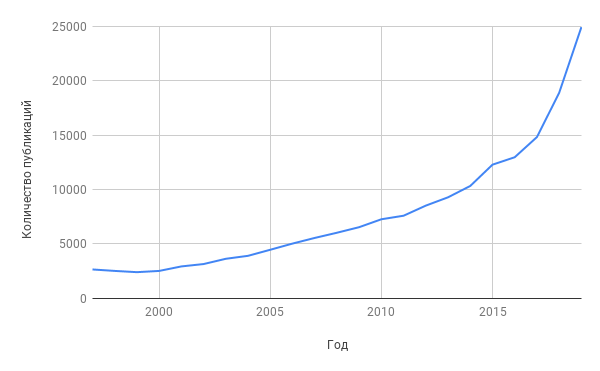
\includegraphics[width=0.8\textwidth]{publications_chart}
\caption{Динамика популярности поисковых запросов. Источник: sciencedirect.com}
\label{fig:publications}
\end{figure}
\begin{figure}[h]
\centering
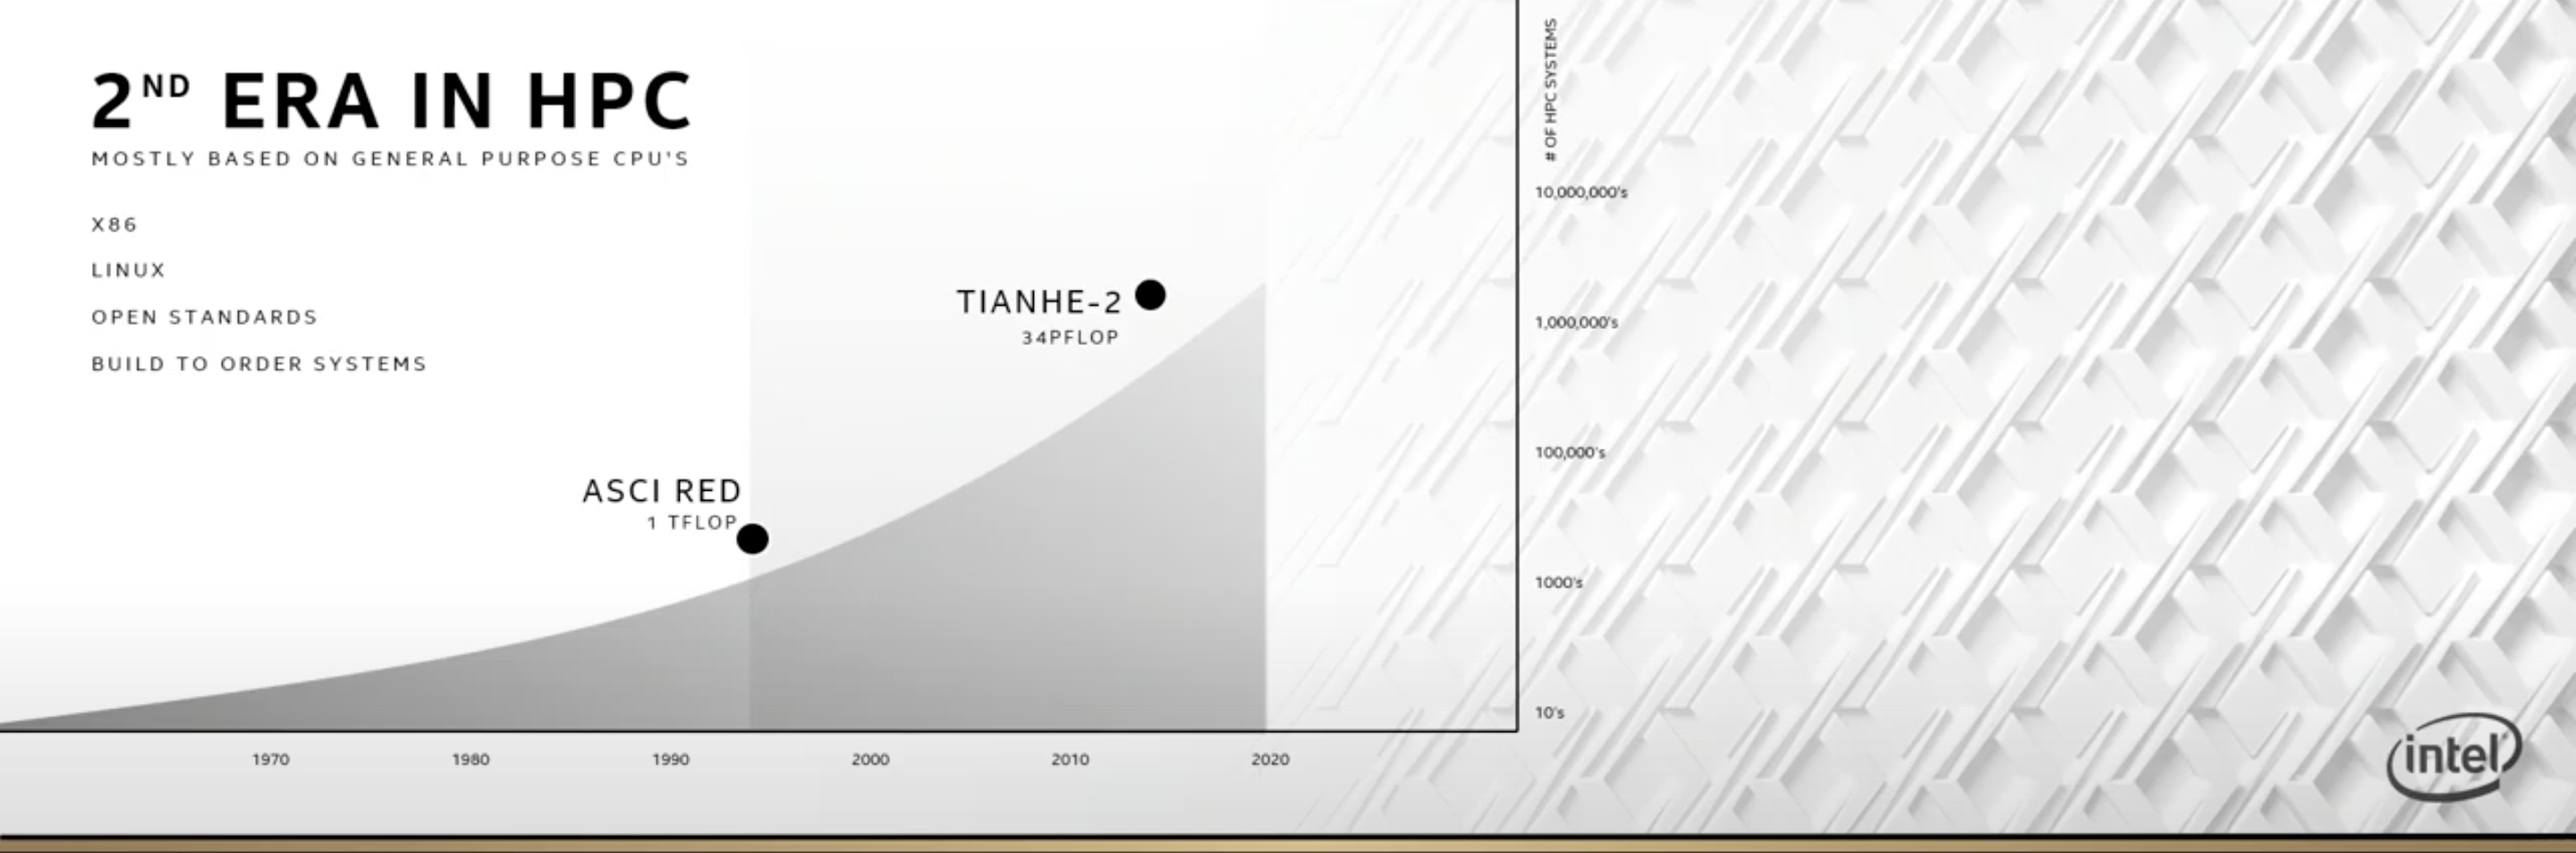
\includegraphics[width=\textwidth]{supercomputer_perf}
\caption{Рост вычислительной мощности суперкомпьютеров. Источник: Intel}
\label{fig:publications}
\end{figure}

Являясь инструментом решения многих прикладных задач, нейронные сети привлекают
не только исследователей, но также бизнес и просто энтузиастов. Чтобы сделать
глубокое обучение более доступным, были разработаны так называемые фреймворки
глубокого обучения -- программные средства, предоставляющие абстракцию над
аппаратным обеспечением. График \ref{fig:search_queries} показывает популярность
различных поисковых запросов. Из него можно видеть, что в то время, как интерес
к технологиям программирования ускорителей падает, растет популярность
фреймворков.
\begin{figure}[h]
\centering
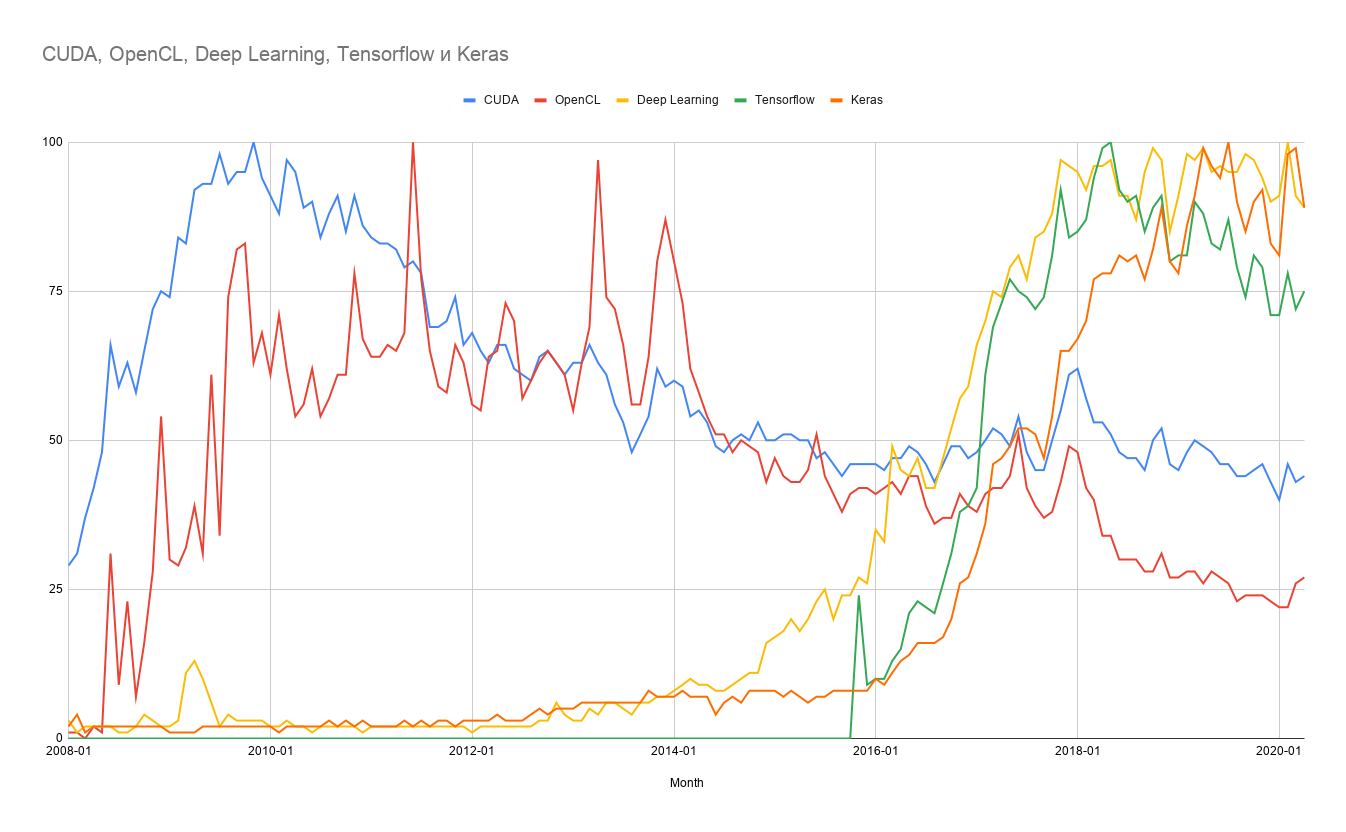
\includegraphics[width=\textwidth]{search_queries}
\caption{Динамика популярности поисковых запросов}
\label{fig:search_queries}
\end{figure}

В то же время, распространенной практикой становится применение компиляторных
технологий в машинном обучении. Это вызвано постоянно растущим количеством
различных ускорителей и аппаратных платформ. Примером таких продуктов могут быть
Glow от Facebook, MLIR и XLA от Google, PlaidML и nGraph от Intel.

Изложенные выше факты говорят об актуальности настоящей работы.

Целью данной работы является исследование применения технологий разработки и
построения компиляторов в задачах машинного обучения.

Исходя из цели работы, поставлены и решены следующие задачи:
\begin{enumerate}
\item Исследование архитектурных особенностей и возможностей современных
      фреймворков для задач искуственного интеллекта;
\item Изучение основных принципов построения современных компиляторов;
\item Разработка компилятора графа вычислений, как базоваого элемента для
      построения фреймворков искусственного интеллекта.
\end{enumerate}

В работе использовались научные труды отечественных и зарубежных специалистов.

Создание компилятора позволит обеспечить вычислительную поддержку математического
аппарата, используемого при построении нейронных сетей, а так же продемонстрировать
ключевые направления развития искусственного интеллекта. Результаты данной
работы в дальнейшем могут использоваться при решении прикладных задач, связанных
с глубоким обучением.

Работа состоит из введения и четырех глав. Первая глава посвящена обзору
научной литературы по тематике исследования. Вторая глава рассматривает основные
архитектурные особенности фреймворков на примере Tensorflow. Третья глава
посвящена современным тенденциям в построении компиляторов, в частности технологиям
LLVM и MLIR. В четвертой главе рассматриваются особенности проектируемой
программной системы.

\clearpage
\section{Обзор литературы}
\subsection{Общие сведения о нейронных сетях}
% todo what is nn
\subsubsection{Многослойный перцептрон}
Описанный Фрэнком Розенблаттом перцептрон -- это линейная модель классификации.
Она делит пространство входов нейронной сети на две части гиперплоскостью.

Перцептрон состоит из элементов трех видов: сенсорные, ассоциативные и
реагирующие. Сенсорные элементы вырабатывают сигнал под воздействием энергии.
Ассоциативные элементы выдают сигнал, когда алгебраическая сумма входящих
сигналов превышает пороговую величину $\theta > 0$. Реагирующий элемент выдает
сигнал $+1$, если сумма входных его сигналов строго положительна, и $-1$, если
сумма входных сигналов строго отрицательная.
\begin{figure}[h]
\centering
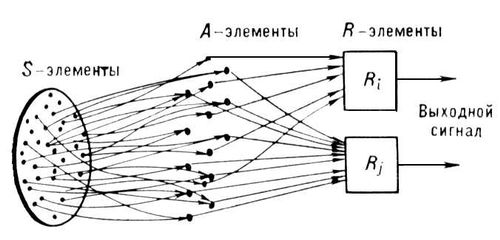
\includegraphics[width=0.5\textwidth]{Perceptron2}
\caption{Перцептрон. Источник: http://www.machinelearning.ru/wiki/index.php?title=Изображение:Perceptron2.jpg}
\label{fig:perceptron}
\end{figure}
\subsubsection{Сверточные нейронные сети}
Сверточные нейнонные сети часто применяются в задачах распознавания образов.
Главной составляющей СНС является слой свертки.

Основная идея сверточной сети -- обработка участка изображения независимо от
его положения. Слой свертки проходит <<окном>> по изображению и пытается
выделить признаки, строя их карту. Более строго этот процесс можно записать
с помощью формулы:
\[
y^{l}_{i, j} = \sum_{-d<=a,b<=d} W_{a,b}x^l_{i + a, j + b},
\]
где $y^l_{i, j}$ -- результат свертки на уровне $l$, а $x^l_{i, j}$ её вход (т.е.
выход предыдущего слоя), $W$ -- матрица весовых коэффициентов\cite{deeplearning}. 
На рисуноке \ref{fig:conv_calc} продемонстрирован пример подсчета результата по 
данной формуле.
\begin{figure}[h]
\centering
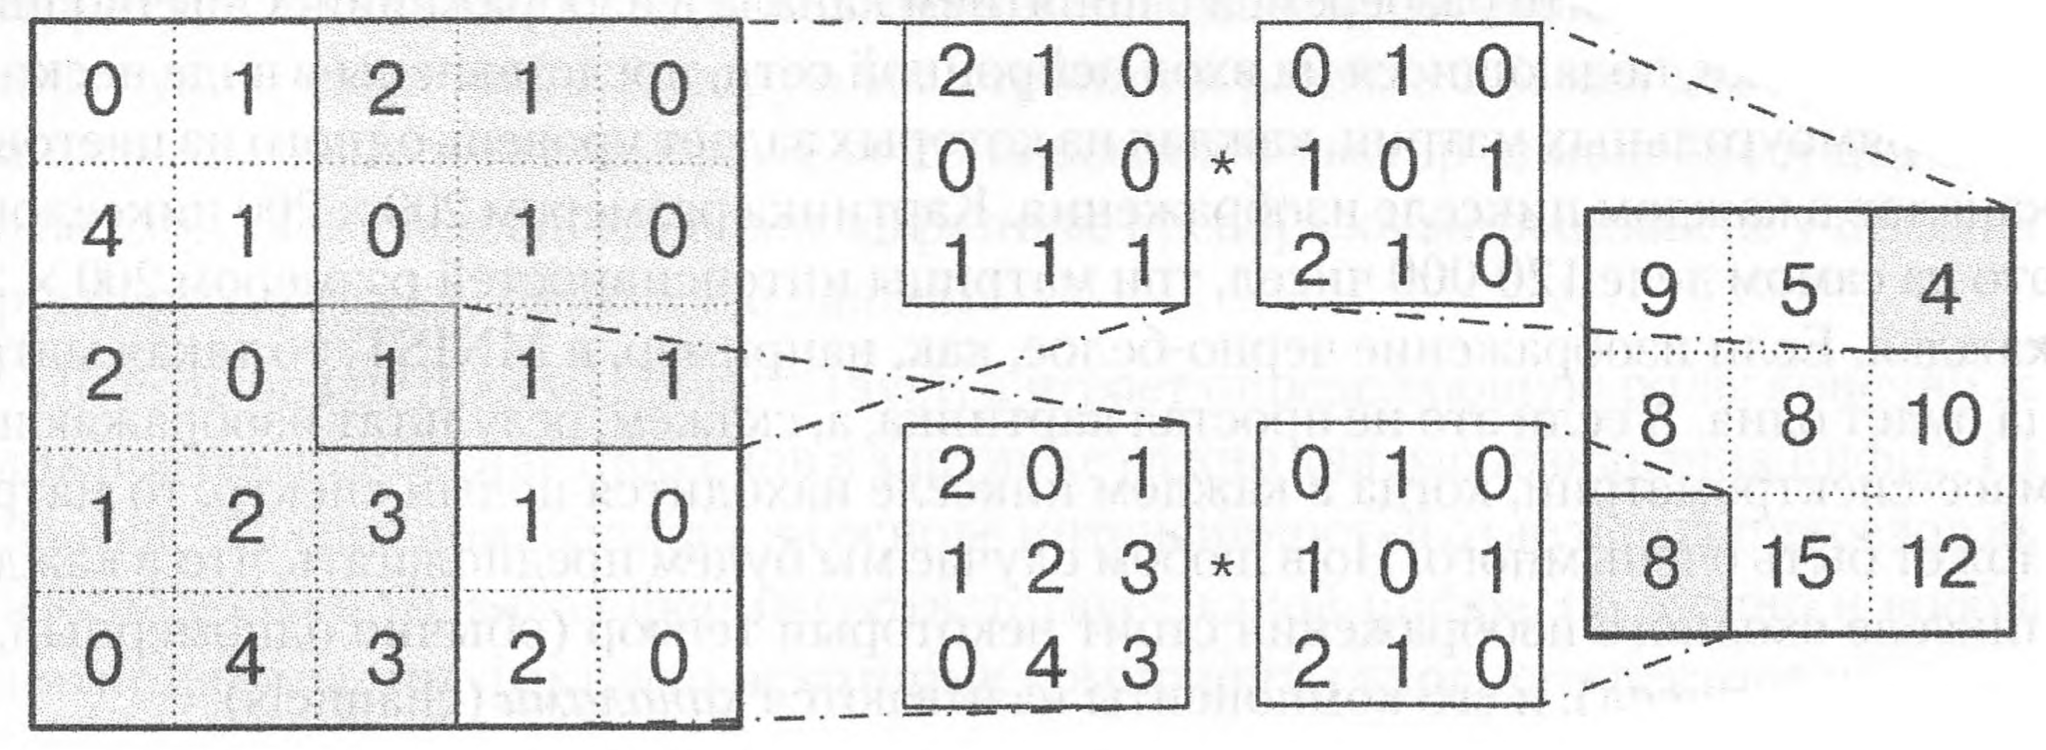
\includegraphics[width=0.8\textwidth]{conv_calc}
\caption{Пример подсчета результата свертки. Источник: \cite{deeplearning}}
\label{fig:conv_calc}
\end{figure}


% todo pooling
% todo LeNet
\subsubsection{Рекуррентные нейронные сети}
Часто исходными данными для нейронных сетей служат последовательности, имеющие
зависимости соседних точек друг от друга. Для выражения такой зависимости
применяются рекуррентные нейронные сети, где связи могут идти не только от
нижнего слоя к верхнему, но и от нейрона к самому себе. 

\begin{figure}[h]
\centering
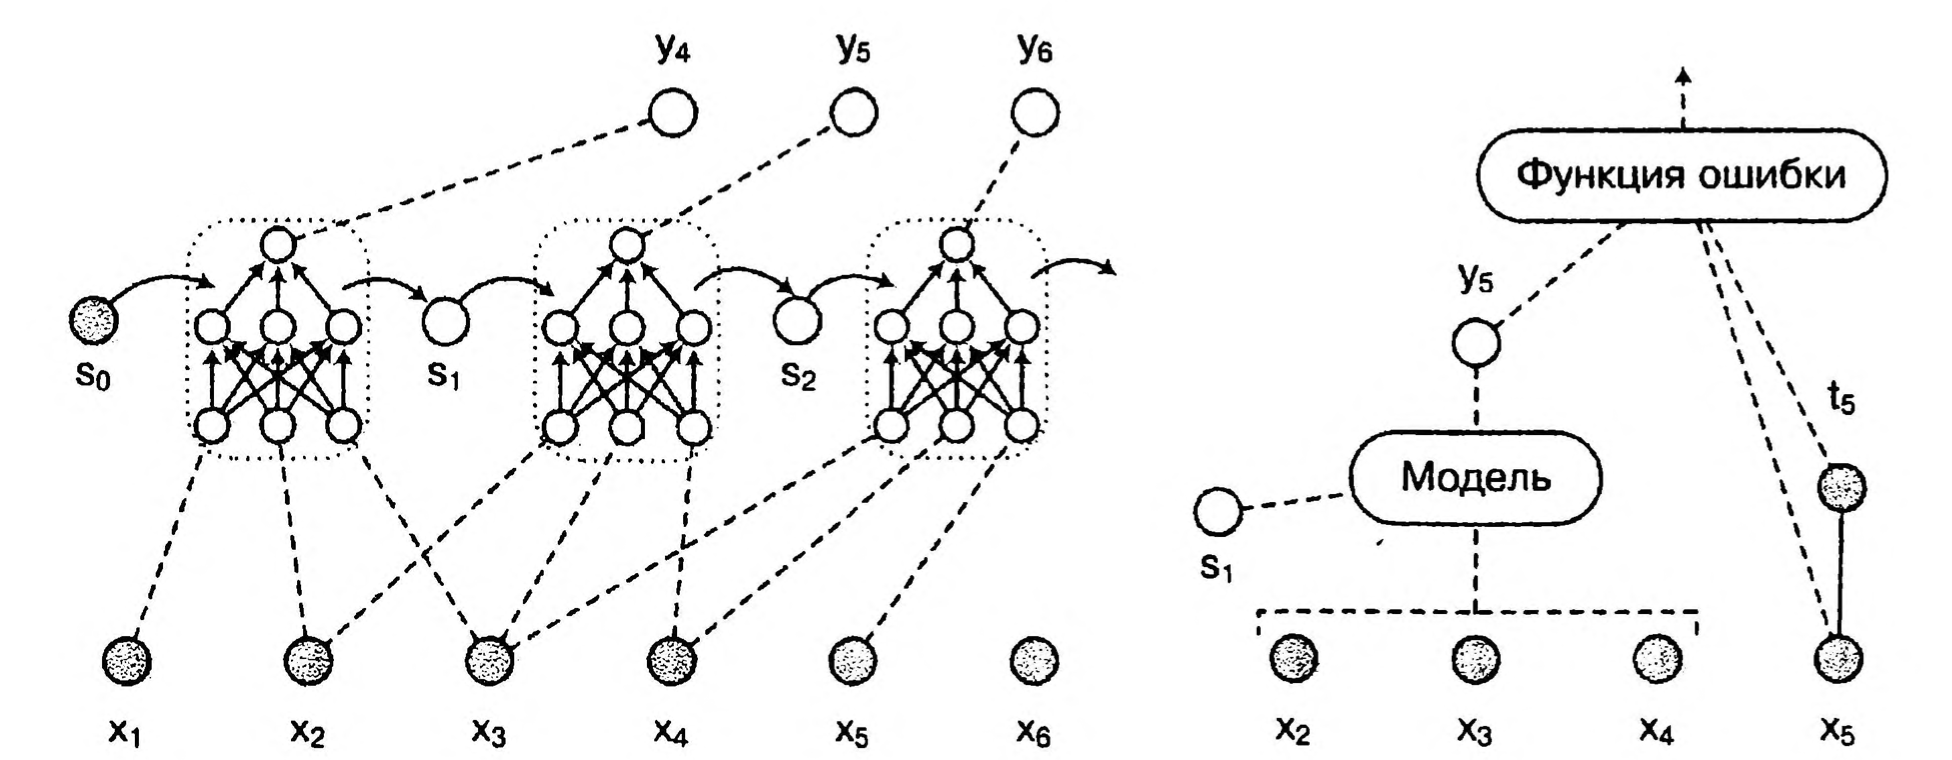
\includegraphics[width=0.8\textwidth]{recurrent_network}
\caption{Рекуррентная нейронная сеть. Источник: \cite{deeplearning}}
\label{fig:recurrent_network}
\end{figure}

На практике часто используется архитектура Long Short-Term Memory (LSTM). Она
состоит из трёх основных видов узлов (вентилей): входной, забывающий и выходной.
На вход ей подаются два вектора: вектор входных данных $x_t$ и вектор скрытого
состояния $h_{t-1}$. Внутри каждого блока есть векторы, выполняющий функцию
памяти (ячейка памяти)\cite{deeplearning}. Это демонстрирует схема на рис. \ref{fig:lstm}.
\begin{figure}[h]
\centering
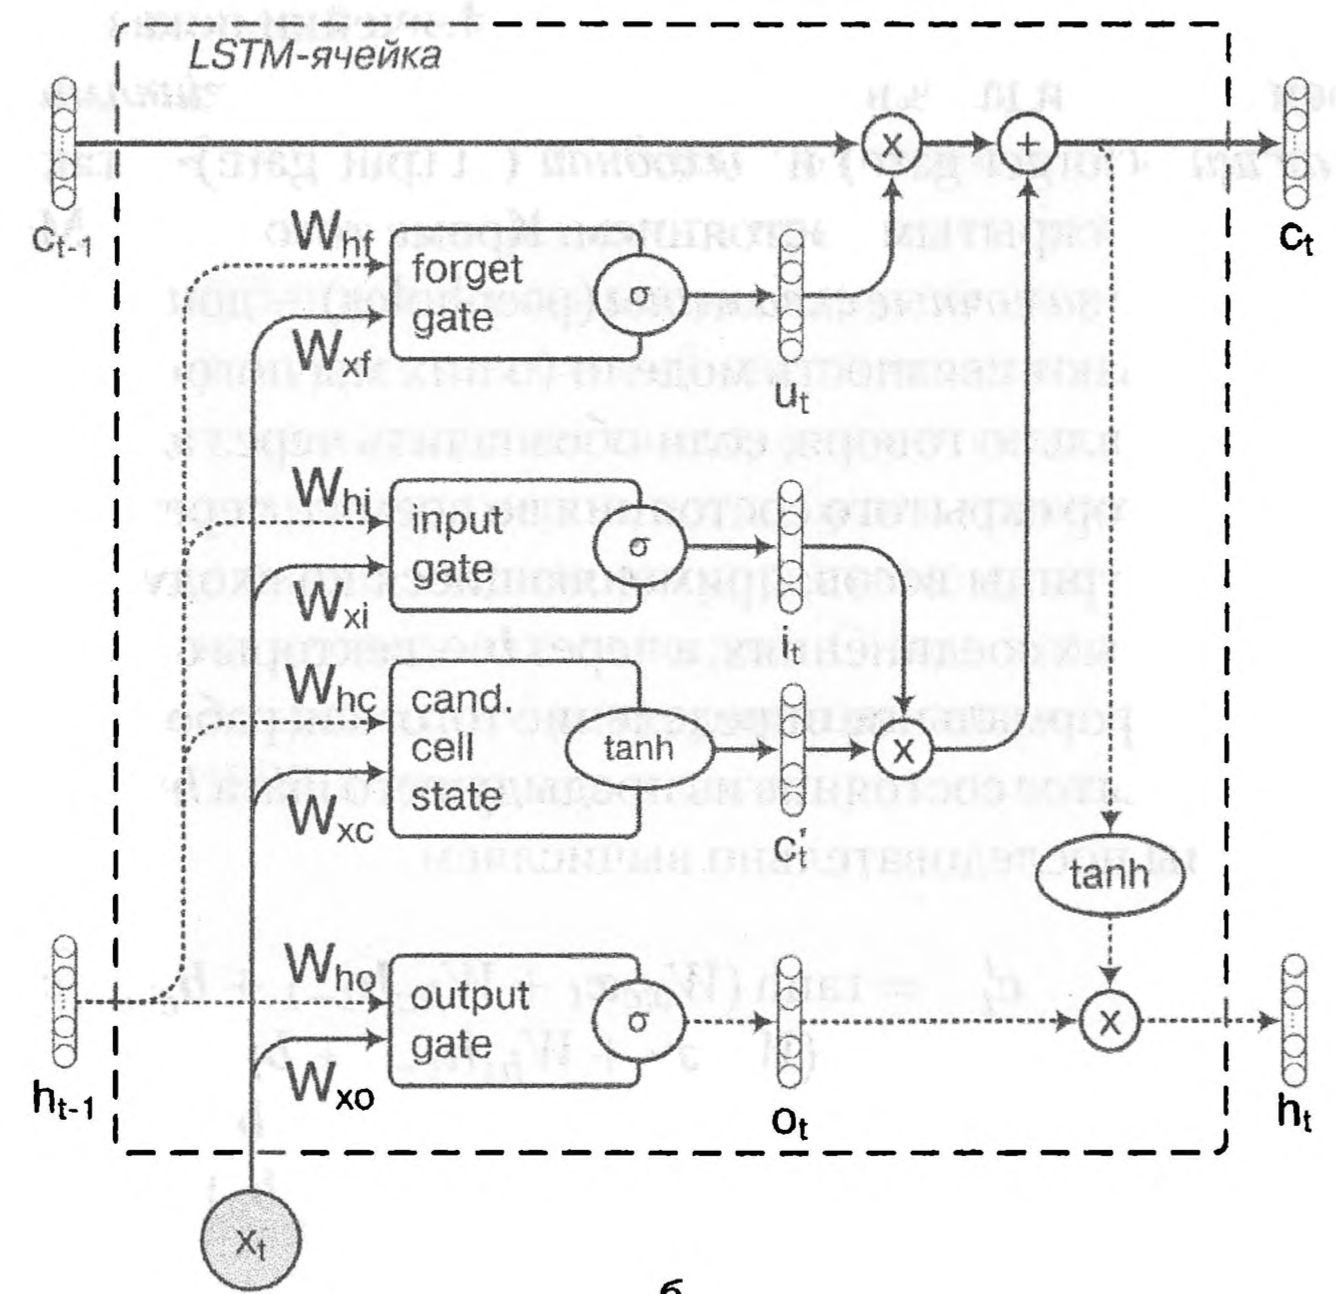
\includegraphics[width=0.8\textwidth]{lstm}
\caption{Ячейка LSTM. Источник: \cite{deeplearning}}
\label{fig:lstm}
\end{figure}

\subsubsection{Метод обратного распространения ошибки}
Метод обратного распространения ошибки -- одна из модификаций классического
градиентного спуска. Основная его идея состоит в распространении сигналов ошибки
от выходов сети к входам в направлении, обратном прямому распространению
сигнала. 
\subsection{Обзор современной литературы}
	Рост популярности искусственного интеллекта привел к появлению большого количества инструментов для исследователей в данной области. В частности, фреймворков. Одним из первых таких фреймворков стал Theano, описанная в статье Rami Al-Rfou et al “Theano: A Python framework for fast computation of mathematical expressions”[4] . Библиотека позволяет определять символьные математические выражения и компилировать их в высоко оптимизированный код для выполнения на CPU и GPU. Выражения представляются в виде графа вычислений - направленного ациклического графа, в котором есть два типа вершин: переменные (variables), содержащие данные, и применяемые (apply nodes), содержащие математические операции. Для дифференцирования графа применяется цепное правило. Также существуют специальные операции, позволяющие управлять потоком выполнения (циклы). Для их дифференцирования применяется техника обратного распространения ошибки во времени, то есть в виде обратного цикла. На этапе обхода графа компилятор может применять к выражению различные оптимизации, например, упрощая выражение, освобождая более не используемые участки памяти.
\par
К сожалению библиотека Theano не обладает возможностями распараллеливания вычислений на кластерах. Решить эту проблему попытались исследователи He Ma, Fei Mao и Graham W. Taylor. В своей статье “Theano-MPI: a Theano-based Distributed Training Framework”[13] они рассмотрели проблемы распараллеливания процесса обучения на нескольких GPU. Графические процессоры могут быть установлены как на локальной машине, так и на удаленной. Чтобы повысить производительность в первом случае, авторы разработали GPU-aware MPI. Данные передаются напрямую от одной видеокарты другой, минуя оперативную память.
\par
Свой фреймворк описали исследователи из Калифорнийского университета в Беркли в статье Yangqing Jia et al “Caffe: Convolutional Architecture for Fast Feature Embedding”[12]. Данные в библиотеке представляются в виде капель (blobs) - четырёхмерных массивов. Данные передаются между слоями, которые принимают одну или несколько капель и возвращают одну или несколько. Выполняется два прохода: прямой, во время которого вычисляется значение функции, и обратный, во время которого вычисляется градиента и корректируются веса. Фреймворк разработан таким образом, чтобы быть модульным и переносимым.
\par
Одним из главных игроков на рынке искусственного интеллекта является Google. В статье Jeffrey Dean et al “Large Scale Distributed Deep Networks”[2] рассматривают некоторые аспекты работы фреймврока DistBelief, предшественника Tensorflow. Исследователи описывают параллелизм двух видов: на уровне данных и на уровне модели. Для тренировки особо крупных моделей фреймворк может разделить граф вычислений на части и выполнять его параллельно на кластере. При распараллеливании данных главной проблемой является оптимизация функции. Классический алгоритм SGD требует вычисления значений функции для всего массива данных. Авторы предлагают модификацию алгоритма под названием Downpour SGD. Базовый принцип его работы таков: данные делятся на части, каждая машина обрабатывает свою порцию независимо, после чего все данные отправляются на сервер параметров, где происходит их слияние. Перед началом обработки каждой новой порции машина загружает с сервера актуальную версию параметров модели.
\par
DistBelief был внутренней разработкой компании. Но в 2015 году Google представила открытую библиотеку Tensorflow. Её устройство описано в статье Martín Abati et al “TensorFlow: Large-Scale Machine Learning on Heterogeneous Systems”[1]. Она многое унаследовала от Theano. Вычисления в фреймворке описываются с помощью графа вычислений, который состоит из набора вершин. Для ветвлений и циклов используются структуры внутри графа. У каждой вершины ноль или более входов и ноль или более выходов. Данные передаются по ребрам графа в виде тензоров - строго типизированных массивов произвольной размерности. Также граф может содержать специальные ребра, управляющие зависимостями. По ним не передаются данные, но они показывают, что вычисление одной вершины должно начаться после завершения вычисления другой. В вершинах графа хранятся операции, у которых есть имя и абстрактное представление вычислений (например, сложение, умножение). У них могут быть атрибуты, которые должны быть предоставлены во время построения графа. С каждой операцией связано ядро - конкретная реализация операции. Клиентские приложения могут взаимодействовать с библиотекой путем создания сессии, которая инкапсулирует в себе граф и методы выполнения вычислений на нем. Она же отвечает за управление многопоточностью. 
\par
Совершенно иной подход предлагают авторы библиотеки Chainer. Она описана в статье Seiya Tokui et al “Chainer: a Next-Generation Open Source Framework for Deep Learning”[8]. Современные фреймворки для глубокого обучения работают по модели Define-and-Run, когда сперва задается граф вычислений, который затем и будет исполняться. Авторы отмечают три проблемы у этого подхода:
\begin{enumerate}
	\item Неэффективное использование памяти. Граф должен оставаться в памяти на протяжении всего процесса обучения. 
	\item Ограниченная расширяемость. Для обеспечения обратной совместимости разработчики не могут расширять модель Define-and-Run, чтобы проектировать более сложные нейронные сети. 
	\item Внутреннее устройство модели недоступно пользователю. Усложняется отладка нейронной сети. 
\end{enumerate}
Чтобы преодолеть эти трудности, авторы представили модель Define-by-Run, когда граф определяется непосредственно в момент его выполнения.
\par
На сегодняшний день большое практическое значение имеет возможность запуска фреймворка на многопоточных и многопроцессорных системах. Этот аспект затрагивают Linpeng Tang, Yida Wang, Theodore L. Willke и Kai Li в статье “Scheduling Computation Graphs of Deep Learning Models on Manycore CPUs”[9]. В статье рассматривается влияние процесса планирования потоков на скорость выполнения графа вычислений в нейронных сетях. Авторы отмечают, что большинство известных фреймворков для машинного обучения используют OpenMP или стандартные средства ОС для управления потоками. Из-за этого возникает ситуация, когда виртуальных потоков запущено больше, чем доступно физических. Частые переключения контекста снижают производительность. Подход авторов заключается в создании некой центральной очереди, куда попадают операции, уже готовые для выполнения. Библиотека сама распределяет элементы очереди по потокам. Во время нескольких первых итераций специальный профилировщик собирает информацию, которая в дальнейшем используется при принятии решений о переключении контекста. В результате авторам удалось получить ускорение от 2,1 до 9,5 раз на 68-ядерном процессоре Intel Xeon Phi при обучении 4 популярных архитектур нейронных сетей. 
\par
Вопросами производительности озадачены и разработчики компании Facebook. В статье Nadav Rotem et al “Glow: Graph Lowering Compiler Techniques for Neural Networks” описывается фреймворк Glow. Glow не является самостоятельной библиотекой для искусственного интеллекта. Она предоставляет возможность компиляции графа вычислений в исполняемый код. Сперва она преобразует граф вычислений в высокоуровневый байткод. Операции разбиваются на более мелкие операции линейной алгебры. Над байткодом производится ряд оптимизаций. Затем генерируется биткод LLVM. Для увеличения переносимости вместе с Glow поставляется стандартная библиотека. Она также преобразуется в биткод LLVM и линкуется с графом. Полученный биткод может быть скомпилирован в машинный код для любой платформы, поддерживаемой LLVM.



\clearpage

\section{Детальный обзор Tensorflow}

В таблице \ref{tbl:comp_table} сравниваются характеристики наиболее
распространенных фреймворков. Из неё видно, что наиболее богатым по функционалу
является фреймворк Tensorflow от компании Google. Он же является наиболее
популярным. Именно поэтому рассмотрение основных архитектурных особенностей
фреймворков для искусственного интеллекта будет производиться на примере Tensorflow.
\begin{sidewaystable}
\caption{Сравнительный обзор фреймворков}
\label{tbl:comp_table}
\begin{tabularx}{\textwidth}{@{}ZZZZZZZ@{}}
\toprule
\textbf{Фреймворк} & \textbf{Лицензия}       & \textbf{Ускорители}                    & \textbf{Модель распределенных вычислений}  & \textbf{Сложность добавления новых операций} & \textbf{Сложность добавления поддержки новой архитектуры} & \textbf{Поддерживаемые ОС}          \\ \midrule
Tensorflow         & Apache 2.0              & CUDA, Google TPU, Qualcomm Hexagon DSP & Сервер параметров                          & Средняя                                      & Высокая                                                   & Windows, Linux, macOS, Android, iOS \\
Caffe              & BSD                     & CUDA                                   & Нет                                        & Высокая                                      & Высокая                                                   & Windows, Linux, macOS               \\
Theano             & Proprietary open source & CUDA                                   & Нет (только с помощью сторонних библиотек) & Низкая                                       & Средняя                                                   & Windows, Linux, macOS               \\
PyTorch            & Proprietary open source & CUDA                                   & Нет (только с помощью сторонних библиотек)  & Средняя                                      & Высокая                                                   & Windows, Linux                      \\
CNTK               & MIT                     & CUDA                                   & Сервер параметров                          & Высокая                                      & Высокая                                                   & Windows, Linux                      \\
Glow               & Apache 2.0              & OpenCL                                 & Нет                                        & Средняя                                      & Низкая                                                    & Windows, Linux, macOS               \\ \bottomrule
\end{tabularx}
\end{sidewaystable}
\subsection{Основные понятия}

В TensorFlow вычисления описываются с помощью графа вычислений (англ.
\textit{computation graph}), который состоит из набора вершин (англ.
\textit{nodes}). У каждой вершины 0 или более входов и 0 или более выходов,
и с каждой вершиной связана операция (англ. \textit{operation}). Значения,
передающиеся по ребрам графа, называются тензорами (англ. \textit{tensor}).
Тензор -- массив произвольной размерности с определенным типом данных элемента.
Кроме того, существуют специальные ребра, называемые зависимостями управления
(англ. \textit{control dependencies}). По ним не передаются данные, но они
показывают, что родительские вершины должны завершить вычисления раньше потомков.

Каждой операции соответствуют имя и абстрактные вычисления (например, умножение
матриц). У операции могут быть атрибуты, значения которых должны быть
предоставлены во время построения графа. Ядром (англ. \textit{kernel}) называют
конкретную реализацию вычислений для определенного класса устройств.

Клиентские программы взаимодействуют с TensorFlow посредством создания сессии
(англ. \textit{session}). Главный метод объекта сессии -- \textbf{Run}. Он
принимает в качестве входных значений имена вершин, значения которых необходимо
вычислить, а так же необходимые для вычисления графа аргументы. Используя эти
данные, TensorFlow может вычислить транзитивное замыкание, содержащее все
вершины, выполнение которых необходимо для получения результата.

Часто граф исполняется несколько раз. Большинство тензоров уничтожается после
исполнения графа. Однако, особый вид операций, называемых переменными (англ.
\textit{variables}), позволяет создать тензоры, которые сохранят свое значение
после исполнения графа.

\subsection{Реализация вычислений}

\subsubsection{Вычисления на графе}

Главными компонентами TensorFlow являются клиент, который использует сессию
для взаимодействия с мастером (англ. \textit{master}), и один или более
рабочих процессов (англ. \textit{worker processes}). Каждый рабочий процесс
управляет одним или более устройством и по указанию мастера исполняет вершины.
Существуют локальная и распределенная реализации интерфейса TensorFlow.
Локальная применяется в том случае, когда мастер, клиент и рабочий процесс
находятся на одной машине. Распределенная позволяет работать в окружении,
состоящем из нескольких машин.

В случае окружения с одним вычислительным устройством оно последовательно
выполняет все вершины с учетом их зависимостей. В частности, каждая
неисполненная вершина хранит счетчик неудовлетворенных зависимостей. Как только
он достигает нулевого значения, вершина добавляется в очередь на исполнение.
По завершении исполнения вершина уменьшает счетчики зависимых вершин на 1.

\begin{figure}[h]
    \centering
    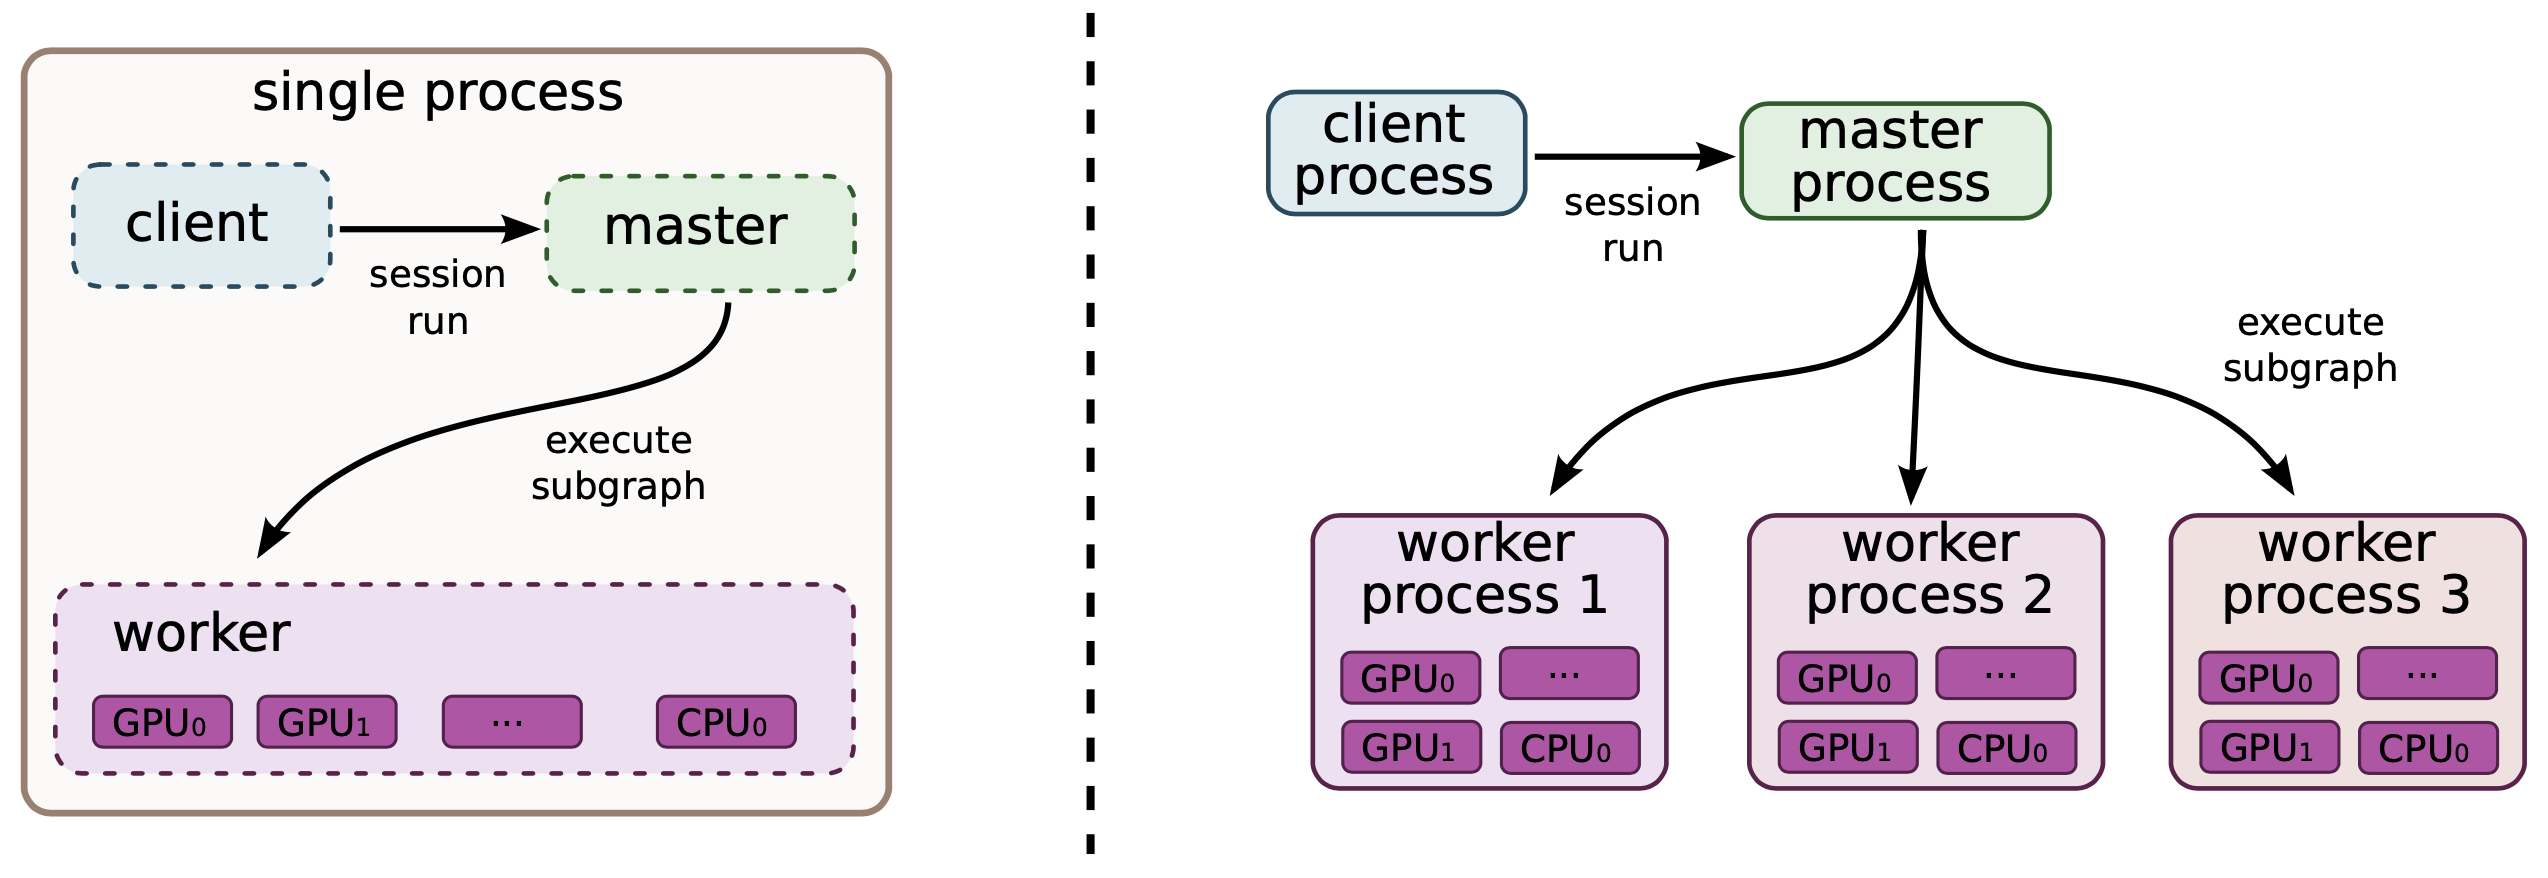
\includegraphics[width=\textwidth]{tf_dev.png}
    \caption{Схема работы TensorFlow с одной и несколькими машинами. Источник \cite{Abadi2016}}
    \label{fig:tf_dev}
\end{figure}

При наличии нескольких вычислительных устройств появляется ряд проблем: принятие
решения о целевом устройстве для каждой вершины, коммуникация между устройствами.

Алгоритм, принимающий решение о размещении вершины на устройстве, учитывает
модель стоимости операций, которая оценивает время исполнения алгоритма и
объем требуемой памяти. Эта модель строится либо на основе эвристик, либо
по результатам предыдущих вычислений. Алгоритм размещения производит симуляцию
вычислений на графе, начиная во входных вершинах и продвигаясь вглубь. Для
каждой вершины, которая рассматривается алгоритмом, определяется список устройств,
на которых она может быть исполнена. В случае, если устройств больше 1,
используется жадный алгоритм, определяющий наиболее подходящее устройство.
Подробнее эти механизмы описаны в разделах 3.2.1 и 4.6 \cite{Abadi2016}.

По окончании размещения вершин происходит деление графа на подграфы. Каждый
подграф выполняется на 1 устройстве. Для обеспечения коммуникации между
устройствами, на границах подграфов вставляются служебные вершины передачи и
приема (англ. \textit{send and receive nodes}).

\begin{figure}[h]
    \centering
    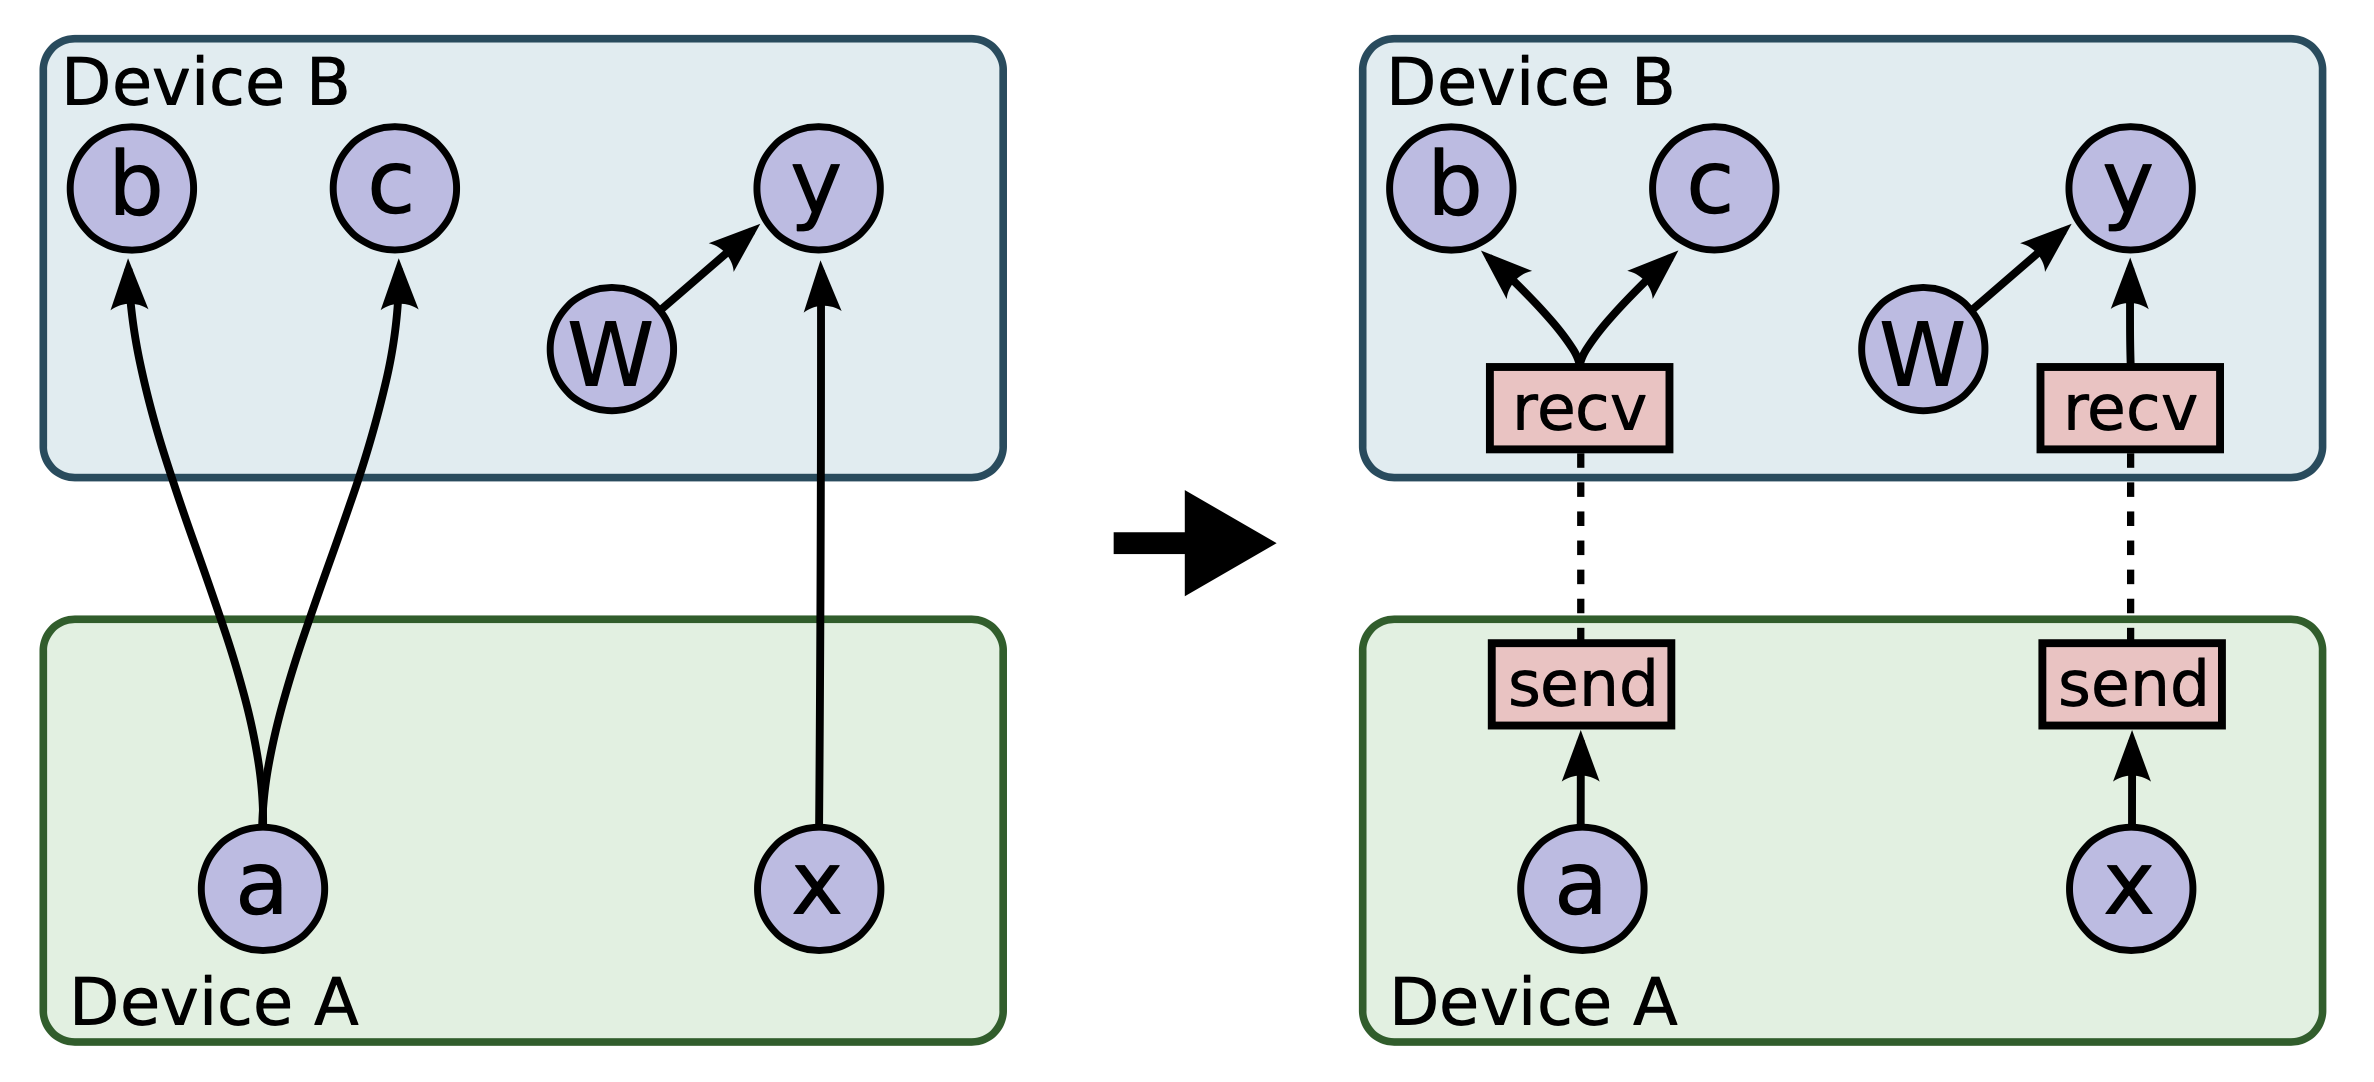
\includegraphics[width=\textwidth]{tf_graph_partition}
    \caption{Граф до и после деления на подграфы. Источник \cite{Abadi2016}}
    \label{fig:tf_graph_partition}
\end{figure}

\subsubsection{Вычисление градиента на графе}

В TensorFlow реализована поддержка автоматического вычисления градиента функции.
Градиент вычисляется так же, как и любые другие функции, путем вычислений на
графе. Для построения необходимого графа используется следующая процедура.

Когда TensorFlow необходимо вычислить градиент тензора $C$ по некоторому
тензору $I$, от которого $C$ зависит, фреймворк сперва находит путь из
$I$ в $C$. Затем, начиная с конца этого пути (то есть из вершины, содержащей $C$),
библиотека добавляет в граф вершину, вычисляющую частную производную,
руководствуясь правилом дифференцирования сложной функции. Каждая операция сама
определяет правила собственного дифференцирования.

\begin{figure}[h]
    \centering
    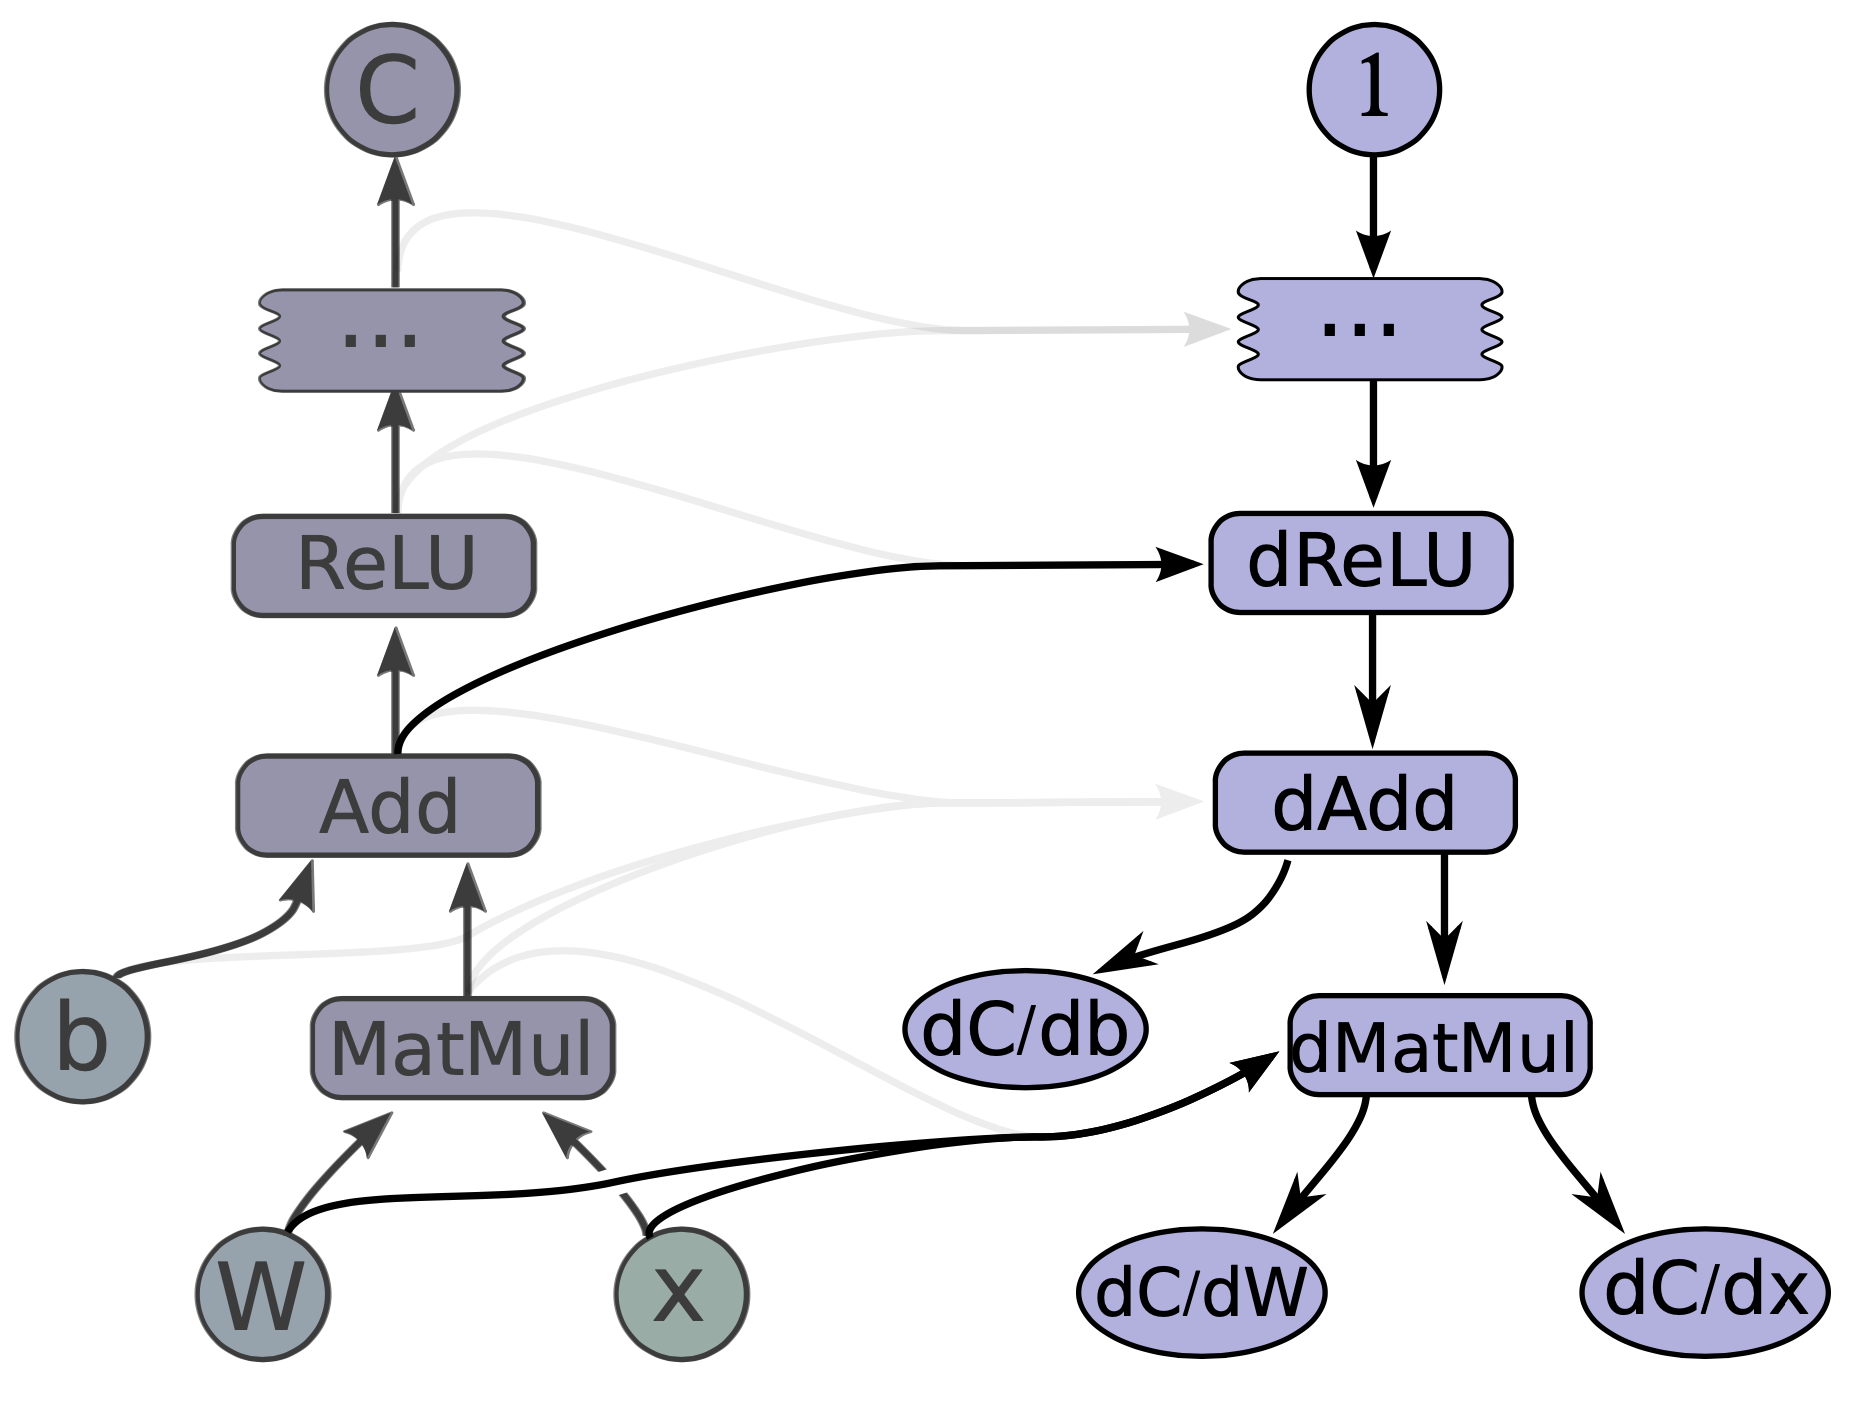
\includegraphics[width=0.5\textwidth]{tf_autograd}
    \caption{Работа алгоритма автоматического дифференцирования. Источник \cite{Abadi2016}}
    \label{fig:tf_autograd}
\end{figure}

В общем случае, у операции может быть несколько выходов, а $C$ может зависеть
только от некоторых из них.

Автоматическое дифференцирование затрудняет работу оптимизационных процедур,
в частности анализ расхода памяти. У пользователя отсутствует возможность
управлять автоматически сгенерированной частью графа. Поскольку градиентные
вершины меняют направление вычислений, тензоры, которые использовались в начале,
зачастую требуются в конце. Это сильно ограничивает размер возможных вычислений,
в особенности на GPU.

\subsubsection{Частичное исполнение}

Часто необходимо вычислить только часть графа. Поэтому фреймворк предоставляет
возможность вычислять только отдельный подграф.

У каждой вершины в графе есть имя, а каждый выход вершины идентифицируется парой
<<имя:порт>>, где порт -- число от 0 до количества выходов. Граф преобразуется
таким образом, что каждая входная пара <<имя:порт>> дополняется вершиной
<<подачи>> (англ. \textit{feed node}), а выходящая -- вершиной <<получения>>
(англ. \textit{fetch node}). Затем используется описанный ранее алгоритм
определения вершин, которые необходимы для вычисления значения графа.

\subsubsection{Управление потоком выполнения}

Концепция управления потоком выполнения в TensorFlow похожа на ту, что
используется в машине потока данных с тегами-токенами MIT (англ.
\textit{MIT tagged-token dataflow machine})\cite{Arvind1987}.
Каждая итерация цикла однозначно идентифицируется меткой (тегом), а состояние
исполнения однозначно описывается фреймом.

В общем случае граф может содержать вершины, принадлежащие разным устройствам.
Таким образом, управление состоянием затрудняется проблемой определения момента
останова цикла. В качестве решения этой проблемы авторы предлагают дополнять
граф специальными управляющими вершинами.

\subsubsection{Операции входных вершин}

Хотя входные данные могут быть предоставлены графу посредством вершин <<подачи>>,
есть другой распространенный механизм, использующийся при обучении больших
распределенных моделей. Обычно таким вершинам предоставляется набор имен файлов.
Во время исполнения они производят один или более тензоров, содержащих образцы
для обучения. Это позволяет загружать данные напрямую с файловой системы. Если
клиент и рабочий процесс находятся на разных машинах, потребуется передача
данных по сети.

\subsection{Оптимизации}

\subsubsection{Выделение общей части выражения}
% todo translation?
Так как построение графа зачастую происходит путем комбинации нескольких слоев,
он может содержать лишние копирования результатов одних и тех же вычислений.
Для оптимизации ресурсов предусмотрен алгоритм выделения общей части выражений.
Этот алгоритм основан на результатах работы \cite{click}.

\subsubsection{Контроль обмена данными и расхода памяти}

Аккуратное размещение вершин на устройствах может привести к значительному
улучшению производительности. В частности, оптимальное планирование может
уменьшить промежуток времени, в течение которого необходимо хранить результаты
промежуточных вычислений.

Наиболее практичным авторы фреймворка видят оптимизацию планирования приемочных
вершин. Они могут начинать исполнение раньше, чем необходимо. Исследователи
анализируют критические пути в графе, чтобы оценить время выполнения вычислений.
Затем граф дополняется управляющими ребрами, откладывающими начало приема данных.

\subsubsection{Сжатие с потерями}

Некоторые алгоритмы машинного обучения, в частности те, что используются в
нейронных сетях, толерантны к шуму и снижению точности вычислений. Авторы
прибегают к сжатию данных с потерями при пересылке между устройствами. Например,
путем конвертации 32-битных чисел с плавающей точкой в 16-битные, а затем
выполняя обратные преобразования. Для этого граф дополняется специальными
вершинами.

\clearpage

\section{Исследование технологий, применяемых для построения компиляторов}

LLVM (первоначально аббревиатура расшифровывалась как Low Level Virtual Machine) начался как
исследовательский проект Университета штата Иллинойс. Целью проекта было разработать промежуточное
представление (intermediate representation, IR), основанное на SSA (single static assignment) 
форме, способное описывать конструкции высокоуровневых языков программирования, а так же
универсальный набор оптимизаций над этим представлением. Неполный список проектов, входящих
в состав LLVM, включает в себя:

\begin{enumerate}
\item Ядро библиотеки, содержащее инструменты для работы с LLVM IR, а так же набор
оптимизаций и трансформаций над ним.
\item Clang -- фронтенд для C, C++ и Objective-C.
\item LLDB -- отладчик для C, C++ и Objective-C программ.
\item libc++ -- имплементация стандартной библиотеки C++.
\item OpenMP -- библиотеки времени исполнения для поддержки стандарта OpenMP.
\item LLD -- линковщик.
\item MLIR -- Multi-Level Intermediate Representation, набор библиотек для
создания собственных высокоуровневых промежуточных представлений и трансформаций
над ними. 
\end{enumerate}

\subsection{Промежуточное представление программного кода}
Static single assignment form (SSA) -- промежуточное представление, в котором
значения переменным присваиваются лишь один раз. Используется компиляторами для
упрощения процесса оптимизации программного кода. Изменяемость переменных может
достигаться двумя путями. Первый -- выделять динамическую память и обновлять
значения операциями чтения и записи в память (\textit{load and store}). Этот
метод использует clang. Однако в таком виде затрудняется статический анализ
памяти (dataflow analysis). Более удобным способом будет добавление суффикса к
имени переменной. В некоторых случаях первая форма может быть приведена ко 
второй с помощью процедуры под названием \textit{memory to register}.
% https://ru.wikipedia.org/wiki/SSA

\subsection{Технологии компиляции исходного кода <<на лету>>}
Компиляция <<на лету>> (англ. \textit{Just-in-time compilation, JIT}) --
один из видов компиляции, когда промежуточное представление программы, 
называемое байт-код, преобразуется в машинные инструкции прямо во время
исполнения программы. В отличие от компиляции перед выполнением (англ. 
\textit{Ahead-of-time compilation, AOT}), JIT позволяет оптимизировать код
программы непосредственно под архитектуру платформы, на которой программа
исполняется, за счет чего достигается повышение производительности. Однако, у
JIT есть недостаток -- увеличенное время запуска программы. В случае, если она
не выполняет сложных вычислений, время запуска и компиляции может превысить 
время работы.
% https://ru.wikipedia.org/wiki/JIT-%D0%BA%D0%BE%D0%BC%D0%BF%D0%B8%D0%BB%D1%8F%D1%86%D0%B8%D1%8F
\subsubsection{Компиляция на основе технологии ORC JIT}
Одна из реализаций JIT компилятора в LLVM носит название ORC (On Request 
Compiler). ORC предоставляет модульный набор программных интерфейсов для 
построения собственных компиляторов. Среди его возможностей:
\begin{enumerate}
\item \textbf{JIT-компоновка} позволяет линковать релоцируемые объекты во время
исполнения программы.
\item \textbf{Компиляция LLVM IR} непосредственно в машинный код.
\item \textbf{Упереждающая и <<ленивая>> компиляция} (англ. \textit{eager and
lazy compilation}). В первом случае вся программа компилируется непосредственно
перед запуском программы и сохраняется в оперативной памяти. Во втором случае
код каждой процедуры компилируется непосредственно перед её вызовом.
\item \textbf{Многопоточная компиляция}.
\end{enumerate}
% https://llvm.org/docs/ORCv2.html

\subsection{Оптимизации программного кода во время компоновки}
Компоновщик -- специальная программа, производящая компоновку (линковку, англ.
\textit{linking}), т.е. связывание бинарных модулей в исполняемый файл.
% https://ru.wikipedia.org/wiki/%D0%9A%D0%BE%D0%BC%D0%BF%D0%BE%D0%BD%D0%BE%D0%B2%D1%89%D0%B8%D0%BA
\subsubsection{Оптимизации с применением технологии ThinLTO}
Оптимизация во время компоновки (англ. \textit{Link time optimization}) -- один
из методов, позволяющий достигать лучшей производительности путем анализа целой
программы (в противоположность классическому анализу единиц трансляции) и
кросс-модульной оптимизации. Во время компиляции вместо машинного кода выдается
промежуточное представление программы, над которым линковщик может совершать
манипуляции.

ThinLTO -- новый подход в LLVM для подобных оптимизаций, впервые представленный
компанией Google в 2015 году\cite{Johnson}.

Процесс компиляции с ThinLTO разделен на 3 фазы:
\begin{enumerate}
  \item \textbf{Компиляция}. Генерация промежуточного представления как полного
        LTO модуля, но дополненного кратким содержанием модулей.
  \item \textbf{Легкая компоновка}. Соединение всех кратких содержаний в единое
        и проведение глобального анализа.
  \item \textbf{ThinLTO backend}. Многопоточные оптимизации с использованием
        данных, полученных на предыдущем шаге.
\end{enumerate}
\begin{figure}[h]
  \centering
  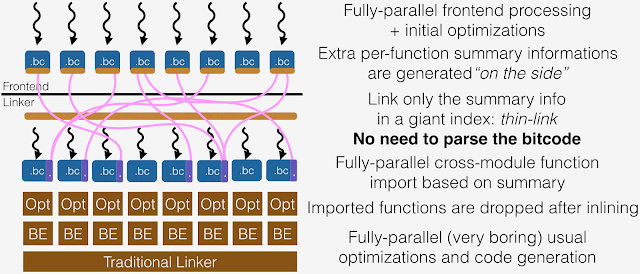
\includegraphics[width=\textwidth]{thinlto.png}
  \caption{ThinLTO. Источник: \url{http://blog.llvm.org/2016/06/thinlto-scalable-and-incremental-lto.html}}
\end{figure}
% https://clang.llvm.org/docs/ThinLTO.html
% http://blog.llvm.org/2016/06/thinlto-scalable-and-incremental-lto.html

\subsection{Исследование инструментов трансляции исходного кода в промежуточное представление}
Проект Clang предоставляет фронтэнд и инфраструктуру для построения инструментов
для работы с C-подобными языками программирования (C, C++, Objective-C,
OpenCL C, CUDA, RenderScript) для LLVM. Благодаря модульной архитектуре, Clang
может выступать не только как компилятор, но и как средство статического анализа
кода, утилита автоматического форматирования, языковой сервер и т.д.

\begin{figure}[h]
  \centering
  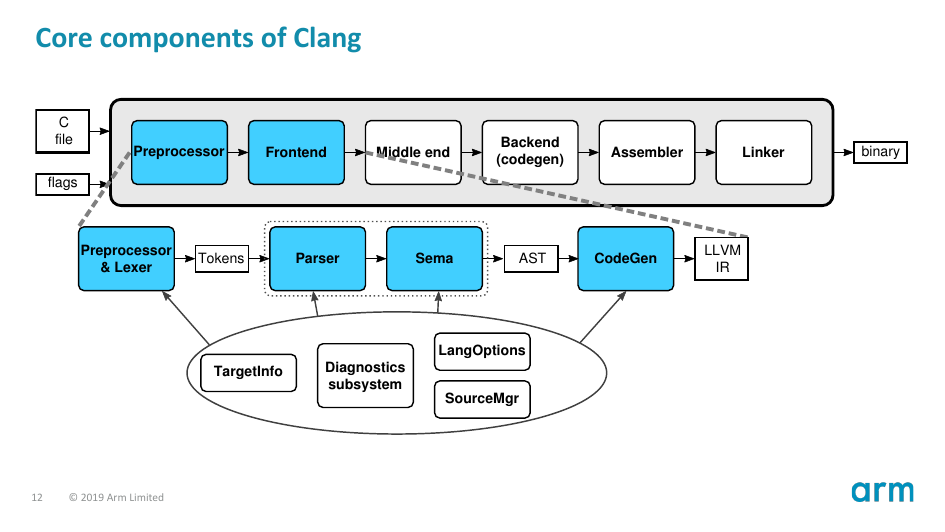
\includegraphics[width=\textwidth]{clangTutorial-18}
  \caption{Ключевые компоненты Clang. Источник: \cite{VanHaagstretSvenARMandStulova2019}}
  \label{fig:clang_core}
\end{figure}
% https://www.youtube.com/watch?v=5kkMpJpIGYU
% http://llvm.org/devmtg/2019-10/talk-abstracts.html#tut8
\subsubsection{Драйвер компилятора и интерфейс командной строки}
Интерфейсом взаимодействия между пользователем и компилятором является драйвер.
Clang предоставляет GCC- и MSVC-совместимые драйверы. Задача драйвера --
распознать аргументы командной строки и сформировать последовательность действий,
которые необходимы для выполнения команды. Основная работа Clang заключается
в выполнении следующей последовательности шагов: чтение файла с исходным текстом,
препроцессинг, разбиение на ключевые слова (англ. \textit{tokens}), лексический
анализ, семантический анализ, генерация абстрактного синтаксического дерева,
генерация LLVM IR (см. рис. \ref{fig:clang_core}).

\subsubsection{Абстрактное синтаксическое дерево}
Абстрактное синтаксическое дерево (англ. \textit{Abstract Syntax Tree, AST}) --
направленный ациклический граф, вершинами которого являются конструкции языка 
программирования (декларации, циклы, операции), а ребрами -- зависимости между
ними. В AST входят не только <<видимые>> конструкции языка, но и служебные,
например, неявное преобразование типов. Это делает подобные деревья хорошей
базой для генерации промежуточного представления. Кроме того, Clang позволяет
превращать AST обратно в исходный код, что позволяет строить на его основе
различные инструменты автоматизации разработки.
\begin{figure}[h]
  \centering
  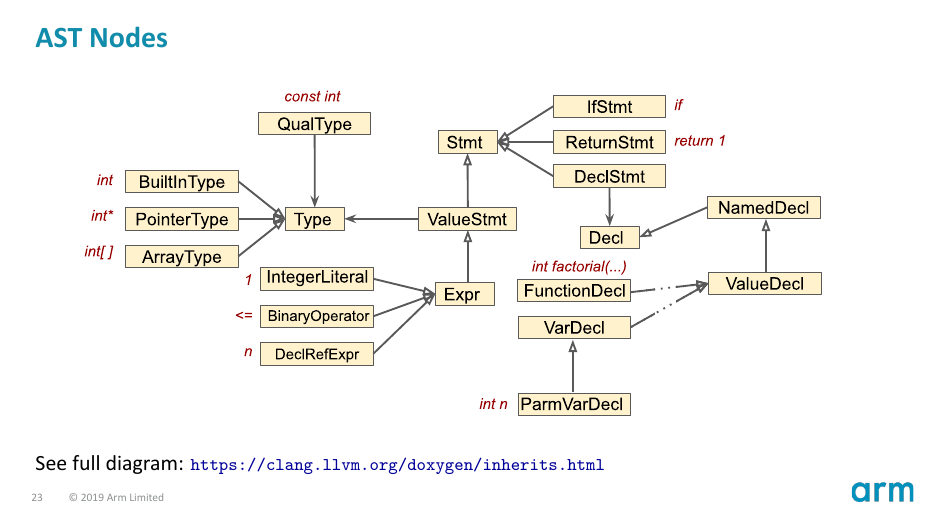
\includegraphics[width=\textwidth]{clangTutorial-48}
  \caption{Основные классы Clang AST. Источник: \cite{VanHaagstretSvenARMandStulova2019}}
  \label{fig:clang_core}
\end{figure}

Ниже представлен исходный код на языке C.
\lstinputlisting[language=C,caption={Пример программы на языке C}]{listings/factorial.c}
Текстовое представление AST для этого фрагмента кода можно увидеть в листинге
\ref{lst:clang_ast} Приложения. На рис. \ref{fig:clang_ast} можно увидеть
графическое представление данного дерева.

\begin{figure}[h]
  \centering
  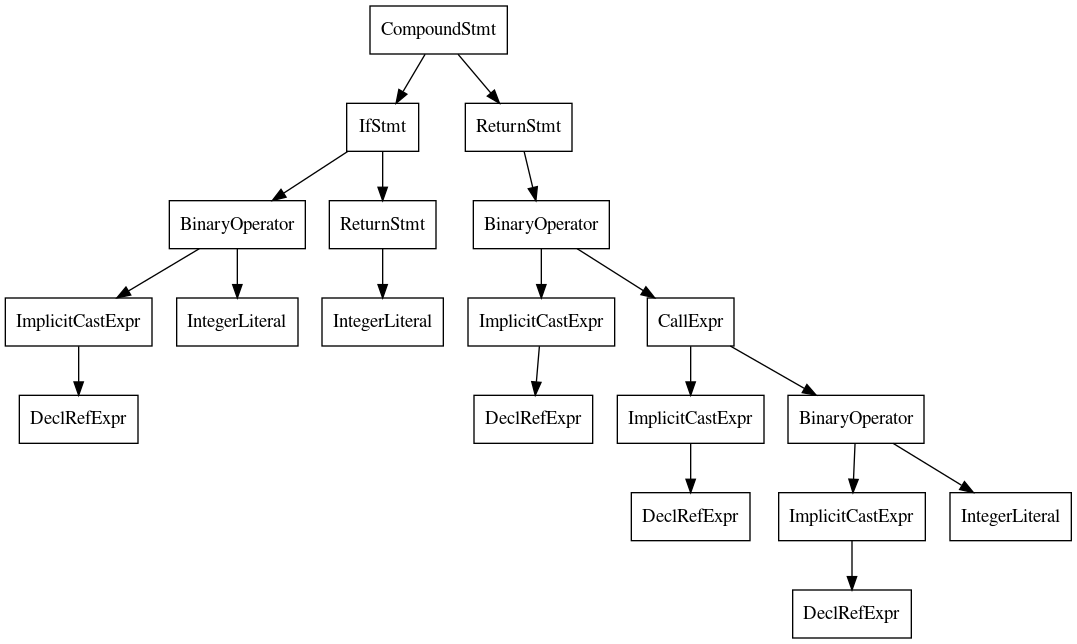
\includegraphics[width=\textwidth]{ast_factorial}
  \caption{Графическое представление Clang AST} 
  \label{fig:clang_ast}
\end{figure}

% TODO example of C function, AST, and AST Graph

\subsubsection{Генерация промежуточного представления из абстрактного синтаксического дерева}
Когда получен AST, компилятор может приступать к генерации кода. В случае с LLVM
перед генерацией машинных инструкций строится описанное ранее промежуточное
представление. Для получения LLVM IR из синтаксического дерева Clang использует
алгоритм обхода графа в глубину. Пример полученного IR можно увидеть в листинге
\ref{lst:llvm_ir_clang} Приложения.

\subsection{Многоуровневое промежуточное представление}
MLIR -- это новая инфраструктура для разработки промежуточных представлений.
По заверениям авторов, ее задача -- борьба с фрагментацией программного
обеспечения, улучшения качества гетерогенной компиляции, уменьшение стоимости
разработки новых компиляторов. MLIR предоставляет инструменты для создания
генераторов кода, трансляторов, оптимизаторов на разных уровнях абстракции\cite{Lattner2020}.
% https://mlir.llvm.org/
% http://llvm.org/devmtg/2019-04/talks.html#Keynote_1
\subsubsection{Диалекты}
Основная идея в MLIR заключается в том, что для разных задач требуется разный
уровень абстракций. В процессе преобразования исходного кода в LLVM IR теряется
информация о конструкциях языка, которая могла бы быть использована для
оптимизации программы. С похожими трудностями сталкиваются разработчики
фреймворков для машинного обучения: в процессе преобразования теряются знания
о предметной области. Основной единицей в MLIR является <<Диалект>> -- набор
типов данных и операций над ними. С помощью диалекта можно описать предметную
область и задать преобразования над этими данными. Кроме того, доступны
механизмы преобразования из одного диалекта в другой. Это позволяет
переиспользовать уже имеющиеся инструменты, переходя от более высокого уровня
абстракции к более низким, когда оптимизации на текущем уровне более невозможны.
Такой стратегии, например, придерживается Tensorflow (рис. \ref{fig:tf_dialects}).
% https://www.youtube.com/watch?v=ff3ngdvUang&feature=youtu.be
\begin{figure}[h]
    \centering
    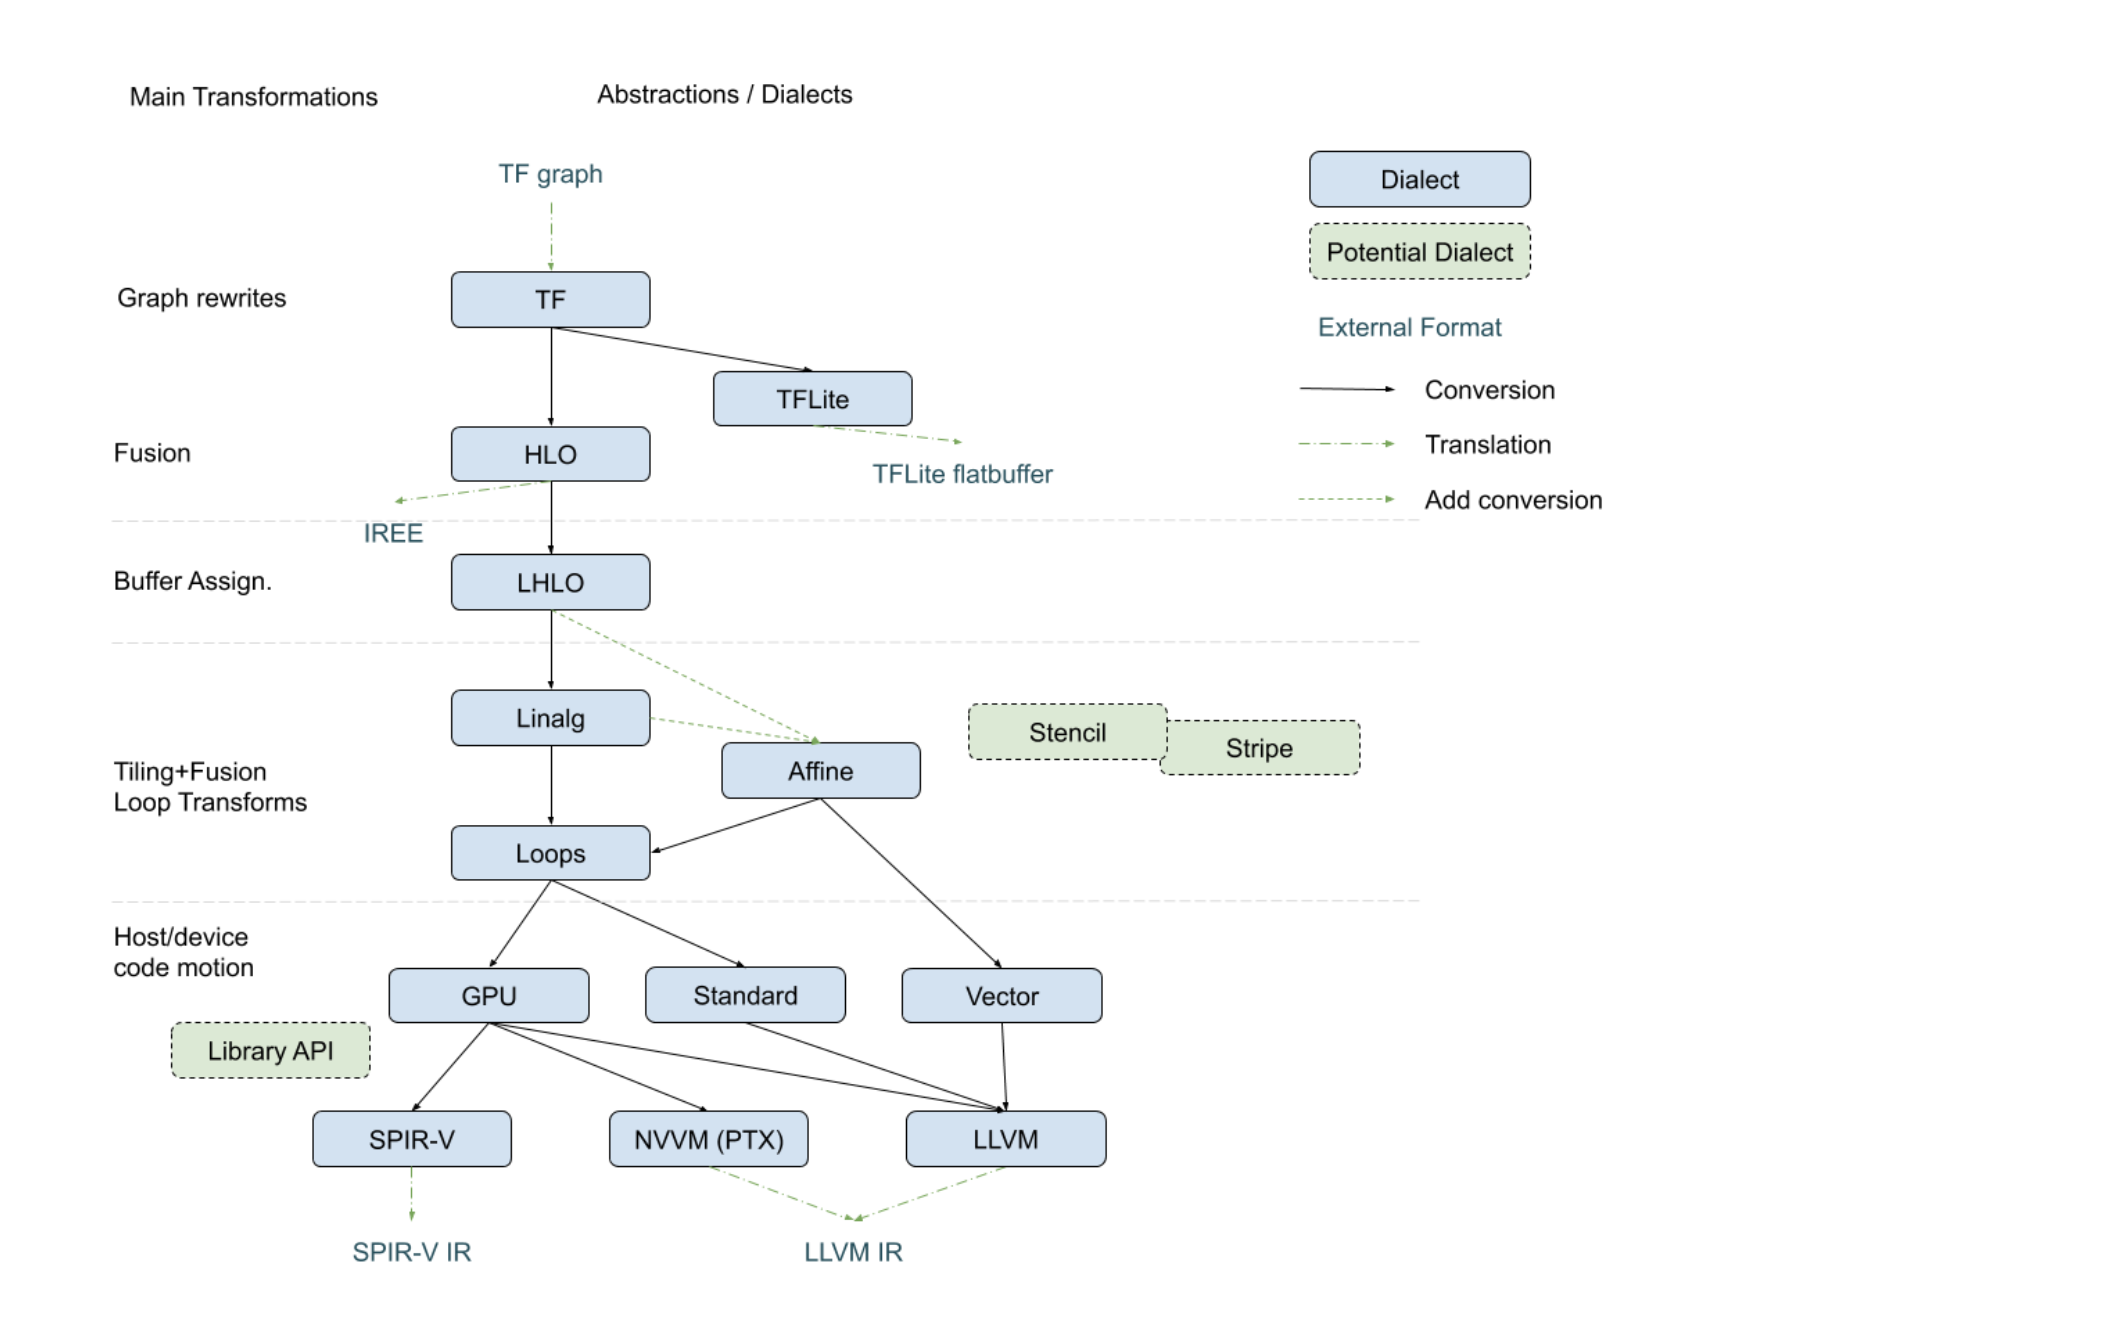
\includegraphics[width=\textwidth]{mlir_vector_dialect.png}
    \caption{Пример взаимодействия диалектов. Источник: \url{https://bit.ly/2YdmVhf}
   % https://docs.google.com/presentation/d/1P-j1GrH6Q5gLBjao0afQ-GfvcAeF-QU4GXXeSy0eJ9I/edit#slide=id.p
    }
    \label{fig:tf_dialects}
\end{figure}
\subsubsection{Упрощенное полиэдральное представление}
Одна из основных конструкций классических языков программирования -- циклы.
Возможность исполнять один и тот же код много раз -- важный инструмент обработки
данных. Его можно сделать еще более гибким, если ввести новую абстракцию и
представить вложенные циклы как аффинное пространство. Любая комбинация
индексных переменных будет точкой в этом пространстве, а множество всех таких
точек -- полиэдром. Используя подобную абстракцию, можно свести оптимизацию
вложенных циклов к аффинным преобразованиям. MLIR предоставляет упрощенное
представление подобных конструкций путем введения в грамматику промежуточного
представления размерностей (англ. \textit{dimensions}) -- идентификаторов,
соответствующих размерности представляемой структуры (т.е. циклов), и символов --
произвольных числовых констант неизвестного происхождения\footnote{\url{https://mlir.llvm.org/docs/Dialects/Affine/}}.
Используя эти данные, фреймворк может выполнять <<склеивание>>,
<<разворачивание>>, векторизацию циклов.

\clearpage

\section{Компилятор графа вычислений}

В рамках данной работы создан компилятор графа вычислений. Проект написан
на языке программирования C++. Исходный код проекта открыт и доступен на
портале GitHub: \url{https://github.com/athenaml/athena}. Схема~\ref{fig:struct}
демострирует структуру основных файлов и каталогов проекта.

\begin{figure}[h]
  \centering
  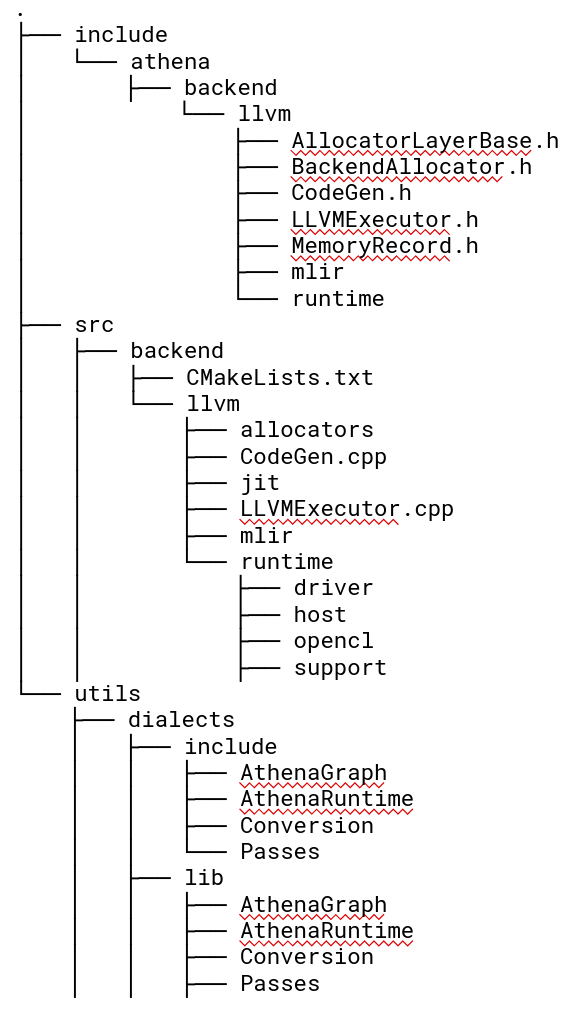
\includegraphics[width=0.4\textwidth]{struct}
  \caption{Структура проекта}
  \label{fig:struct}
\end{figure}

Общая схема работы компилятора представлена на рис.~\ref{fig:compiler_scheme}. 
На вход ему поступает граф вычислений. Затем последний преобразуется в код на языке
диалекта высокого уровня. Этот код подвергается различным оптимизациям и
преобразованиям, после чего транслируется (<<понижается>>) в код на языке
диалекта низкого уровня. После очередной итерации преобразований низкоуровневый
диалект преобразуется в LLVM IR и передается в JIT-компилятор для генерации
машинного кода и исполнения. Полученный исполняемый модуль содержит вызовы к
библиотеке среды исполнения, которая отвечает за взаимодействие с физическими
устройствами и управление памятью.

\begin{figure}[h]
  \centering
  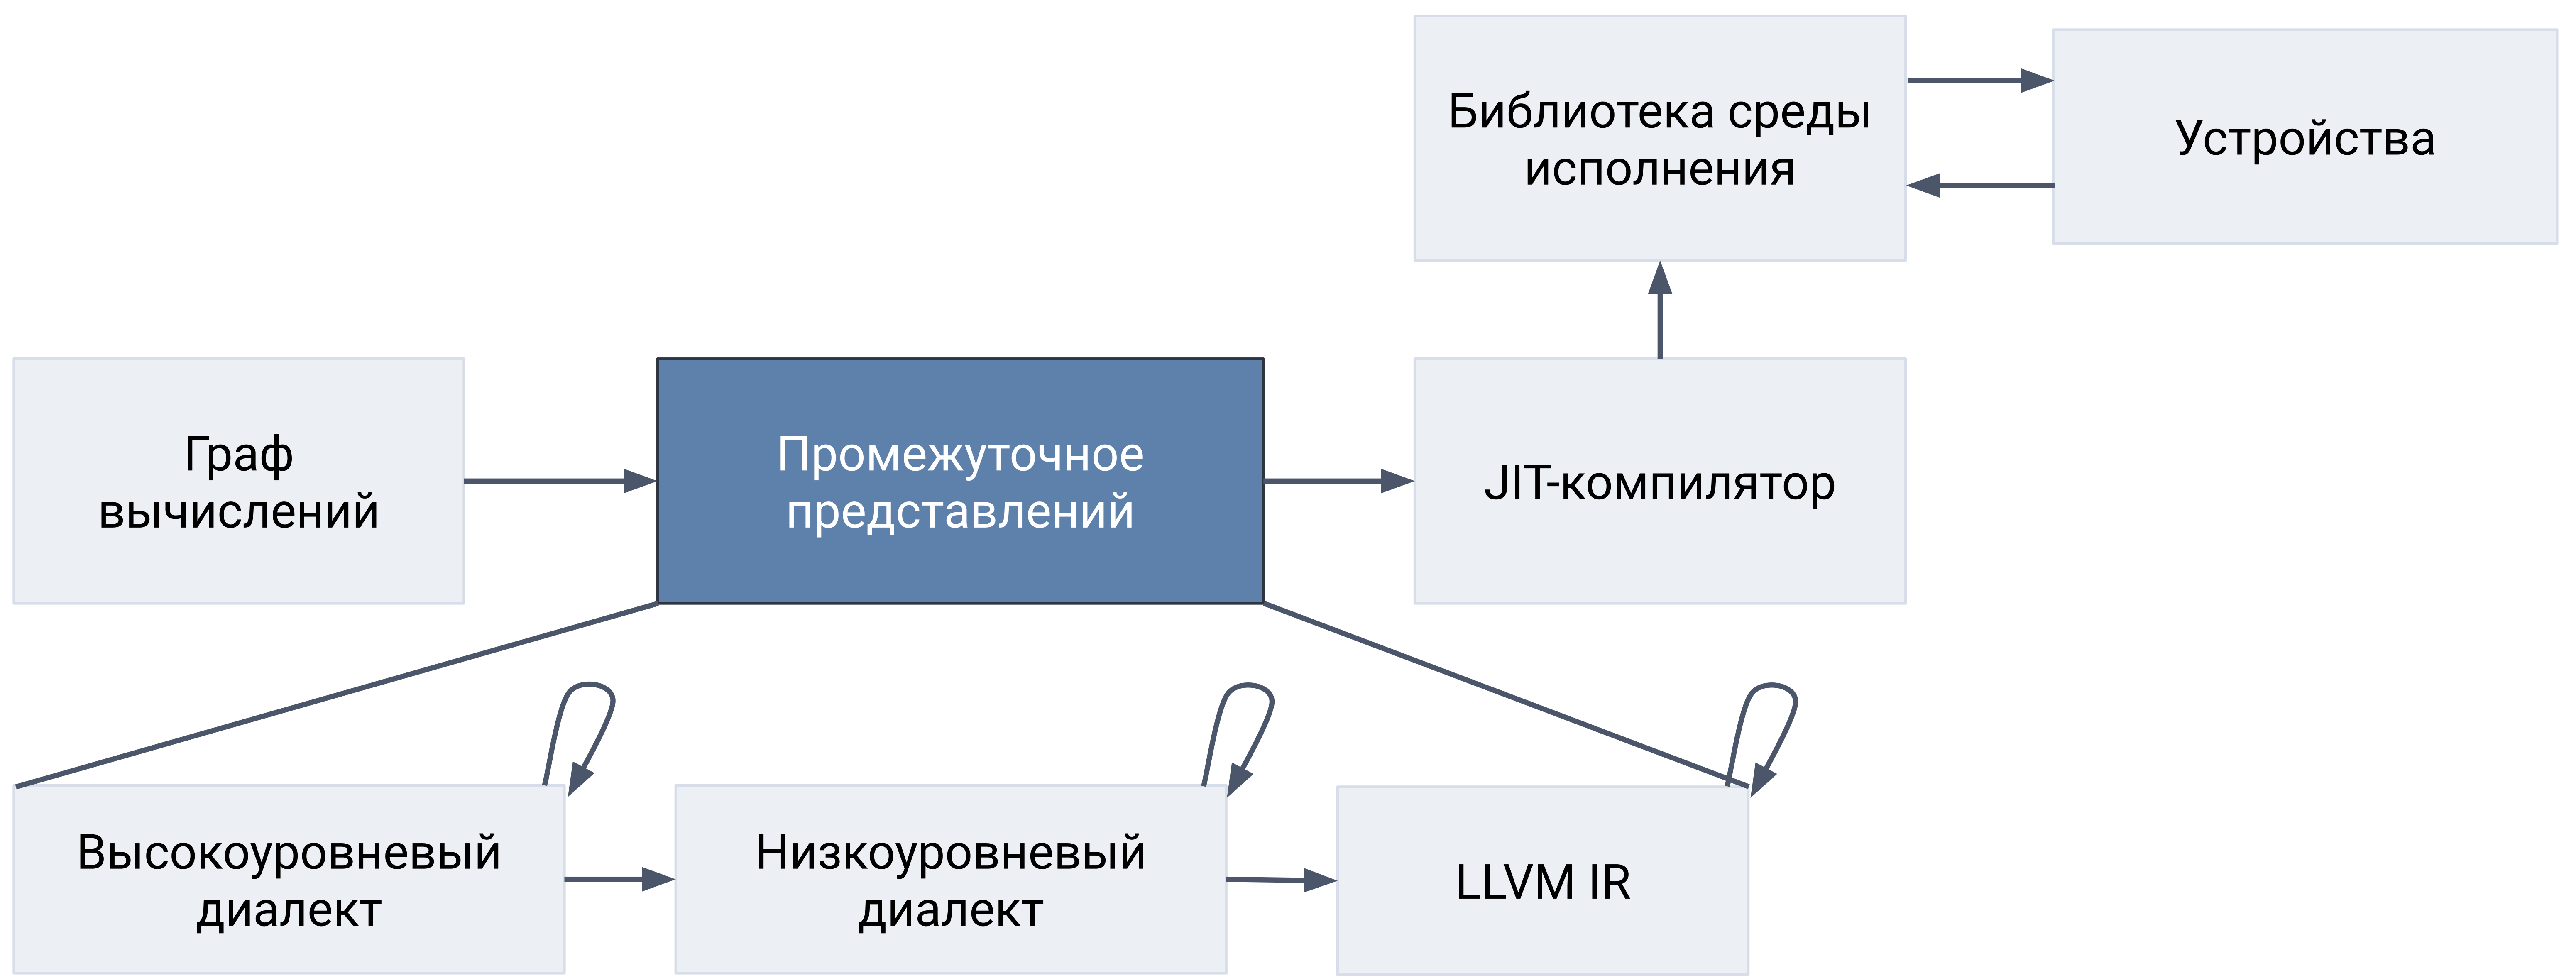
\includegraphics[width=\textwidth]{compiler_scheme}
  \caption{Схема работы компилятора графа вычислений}
  \label{fig:compiler_scheme}
\end{figure}
\subsection{Граф вычислений}

Рассмотрим пример простейшей функции:
\[
  f(x, y) = x + y.
\]
В простейшем случае можно представить эту функцию с помощью графа вычислений,
изображенного на рис.~\ref{fig:simple_add}. В то же время, существует множество
нюансов, о которых необходимо позаботиться, при вычислении данной функции.
Однозначно определить операцию сложения можно лишь для объектов (скаляров,
векторов, матриц, тензоров) одинаковых размеров и одинаковых типов данных.
Кроме того, необходимо позаботиться о выделении нужного объема памяти для
выполнения операции. Таким образом, граф должен включать в себя инофрмацию не
только о математических операциях, но и информацию о природе входных данных. 

\begin{figure}[h]
  \begin{subfigure}{.3\textwidth}
    \centering
    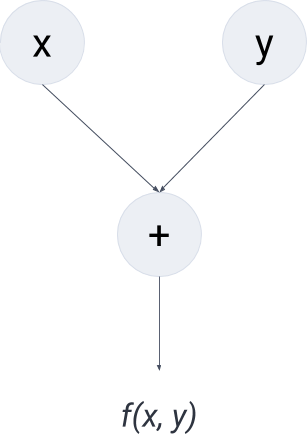
\includegraphics[width=0.8\linewidth]{simple_add}
    \caption{В простейшем случае}
    \label{fig:simple_add}
  \end{subfigure}
  \begin{subfigure}{.7\textwidth}
    \centering
    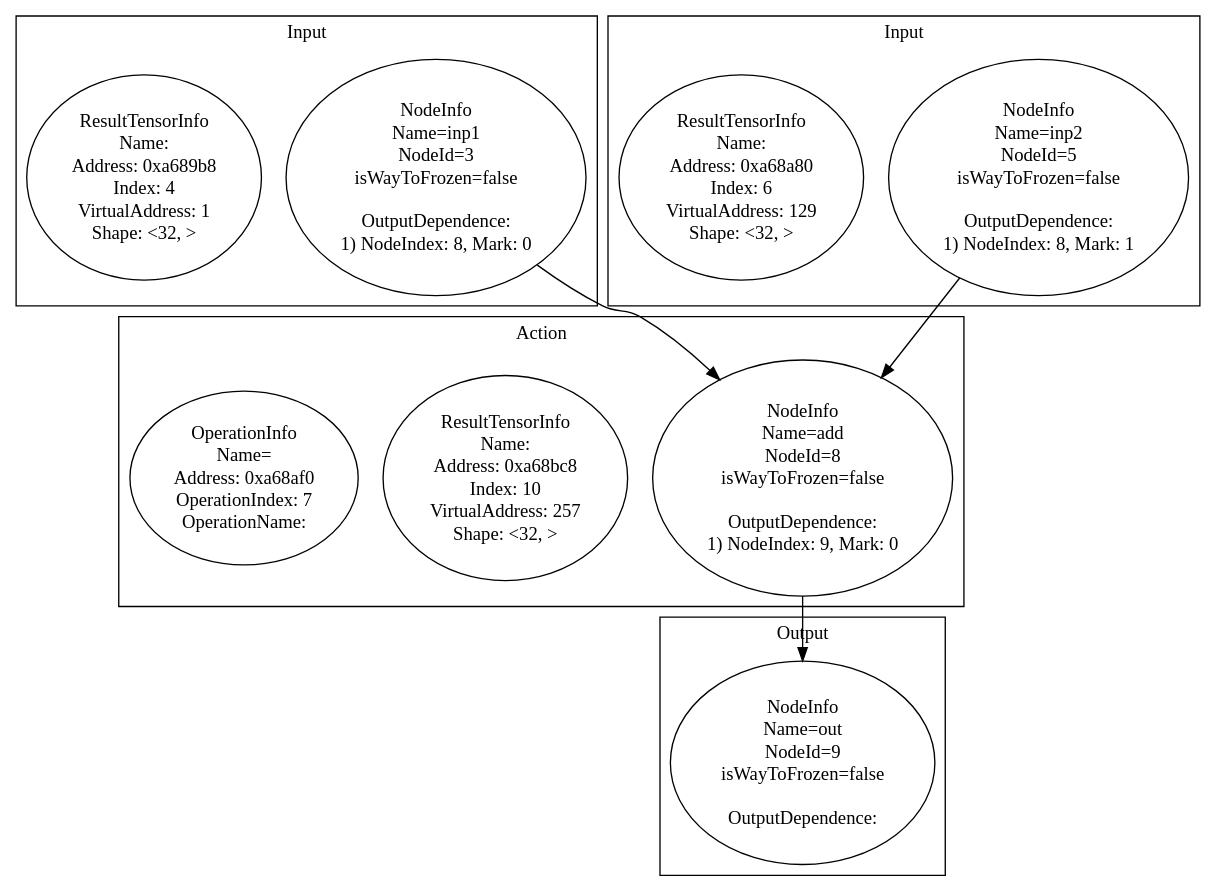
\includegraphics[width=\linewidth]{advanced_add}
    \caption{С учетом дополнительной информации}
    \label{fig:advanced_add}
  \end{subfigure}
  \caption{Пример графа вычислений для функции $f(x, y) = x + y$}
  \label{fig:add}
\end{figure}


Именно это показано на рис.~\ref{fig:advanced_add}. Такой граф содержит
информацию о типе вершины (входная, выходная, вычисления), размерность и тип
данных тензора, виртуальный адрес тензора и т.д. Этой инофрмации достаточно
для генерации исплняемого кода.

Чтобы выполнить преобразование, граф вычислений сперва разбивается на 
кластеры\footnote{Более подробно структура графа и алгоритм разбиения на кластеры
рассматриваются в работе \cite{graph}} таким образом, что вершины каждого нового кластера
зависят только от результатов вычислений вершин в предыдущих кластерах. Таоке
разбиение дает ряд преимуществ. Во-первых, вершины в пределах одного кластера
независимы, а значит их можно вычислять одновременно. Во-вторых, при обработке
кластеров можно так же добиться параллелизма. После того, как кластер $n$
закончил работу и передал следующему кластеру, он может вернуться к работе,
обрабатывая очередную порцию данных. В-третьих, упрощается преобразование графа
в код. Данная трансформация выполняется путем последовательного обхода кластеров
и генерации кода для принадлежащих ему вершин.

\subsection{Высокоуровневый диалект}
Задача высокоуровневого диалекта -- представить граф вычислений в доступном для
компилятора виде, сохранив при этом смысловую информацию о вычислениях.

Для моделирования данного диалекта будет использоваться описанная ранее
технология MLIR. С ее помощью будет сконструирован язык, похожий по свойствам
на язык LLVM IR, а так же разработаны инструментальные средства обработки
полученного промежуточного представления.

Основными компонентами программы на языке диалекта высокого уровня являются
вершины и графы. По своим свойствам они напоминают функции. Вершины могут 
принимать и возвращать значения. Графы же больше походят на функцию main и 
имеют строго определенную сигнатуру: не принимают и не возвращают значений.
Из тела <<функции>> графа происходят вызовы функций, вычисляющих вершины.
Кроме того, в графе содержатся специальные операции -- барьерные синхронизации.
Достигая такой операции, программа приостанавливает работу до завершения
начатых ранее вычислений. Вершины же описывают действия, которые необходимо
совершить для получения корректного результата. К ним относятся выделение памяти,
загрузка данных в память, математические операции, совершаемые над тензорами.

Помимо привычных типов данных, таких как целое число или число с плавающей
точкой, вводится специальный тип данных <<тензор>>. Тензор характеризуется
своей размерностью и типом данных элемента тензора. Размерность тензора может
быть не определена в момент построения промежуточного представления, но должна
быть выведена в ходе последующих преобразований.

\begin{lstlisting}[language=athgraph,caption=Различные варианты тензоров]
%0 = "ath_graph.create_tensor"() {virtual_address = 1 : index} : () -> tensor<2x2xf32> // Матрица 2x2
%1 = "ath_graph.create_tensor"() {virtual_address = 5 : index} : () -> tensor<?xf32> // Вектор неизвестной длины
%2 = "ath_graph.create_tensor"() {virtual_address = 9 : index} : () -> tensor<*xf32> // Тензор неизвестного ранга
\end{lstlisting}

Пример кода, полученного в результате компиляции графа для функции 
$f(x, y) = x + y$, приведен в листинге~\ref{lst:ath_graph_add} Приложения 1.

Поскольку высокоуровневый диалект содержит информацию о семантике вычислений,
возможен ряд высокоуровневых преобразований. Например, операция транспонирования,
примененная дважды к одной и той же матрице, не имеет никакого эффекта, а значит
может быть опущена. С другой стороны, многие математические библиотеки
предоставляют функцию умножения матриц с предварительным транспонированием.
То есть операцию транспонирования и последующее матричное умножение можно
заменить единой операцией, сократив количество обращений к памяти.

\subsection{Низкоуровневый диалект}

После того, как все возможные оптимизации были применены к графу, можно
постепенно переходить к генерации исполняемого кода. Делается это в три этапа.
Сперва промежуточное представление высокого уровня понижается до низкоуровневого
диалекта. Затем он преобразуется в LLVM IR, который и будет скомпилирован
в машинные инструкции.

Задача низкоуровневого диалекта -- помочь среде времени исполнения оптимально
распределить нагрузку, сохранив правильный порядок выполнения операций.

В рамках низкоуровневого диалекта происходит переход от зависимости по данным
к зависимости по событиям (англ. \textit{event}). Вершины и графы заменяются 
обычными функциями. Все инструкции, отвечающие за выполнение математических 
операций, заменяются инструкциями, выполняющими запуск тех или иных 
вычислительных ядер (англ. \textit{kernel}). Кроме того, низокуровневый диалект
предоставляет информацию об итерационном пространстве
(англ. \textit{index space}), в котором происходит выполнение ядра.

Термины ядро и итерационное пространство здесь и далее употребляются в том же
смысле, что и в спецификации стандарта OpenCL. Ядро -- функция, которая
выполняется на физическом устройстве (CPU, GPU, FPGA). Итерационное пространство
-- $N$-мерное пространство (где $N \in {1, 2, 3}$), в котором выполняются ядра
(рис.~\ref{fig:index_space}).

\begin{figure}[h]
  \centering
  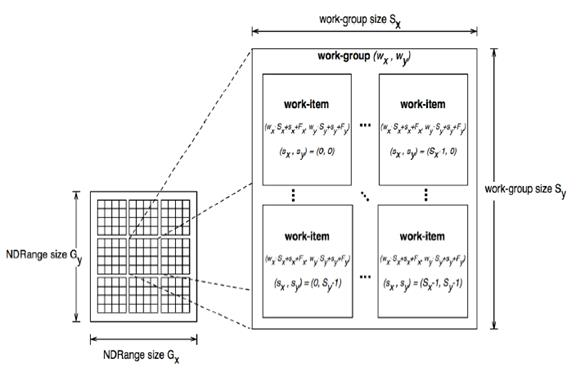
\includegraphics[width=0.8\textwidth]{index_space}
  \caption{Итерационное пространство в OpenCL. Источник: \cite{opencl3}}
  \label{fig:index_space}
\end{figure}

Низкоуровневый диалект вводит три новых типа данных: описание графа
(англ. \textit{Graph handle}), устройство (англ. \textit{device})
и событие (англ. \textit{event}). Описание графа -- указатель на специальную
структуру, которая содержит служебную информацию, например, список доступных
устройств. Устройство -- указатель на стуктуру, содержащую описание физического
устройства, на котором будет выполнено ядро. Событие -- указатель на структуру,
содержащую информацию о конкретном запуске ядра.

Результаты преобразования можно увидеть в листинге~\ref{lst:ath_rt_add} Приложения 1.

Дальнейшее понижение в LLVM IR подразумевает построение специальной структуры
данных, которая содержит в себе информацию об имени ядра, порядке и размерах
входных аргументов и итерационном пространстве. Именно она и передается
в библиотеку времени исполнения.

Полученный LLVM IR представлен в листинге~\ref{lst:llvm_add} Приложения 1.

Трансляция из одного диалекта в другой выполняется за счет стандартных средств
MLIR. Существует три вида конверсий:

\begin{enumerate}
  \item \textbf{Частичная} конверсия допускает, что некоторые операции исходного
  диалекта не могут быть преобразованы в целевой и будут оставлены без изменений.
  \item \textbf{Полная} конверсия требует преобразования всех операций. Если
  не удалось преобразовать хотя бы одну операцию, процедура считается неудачной.
  \item \textbf{Аналитическая} конверсия не выполняет реальных преобразований
  и лишь служит для получения отчета о том, какие операции исходного диалекта
  могут быть преобразованы в целевой.
\end{enumerate}
При этом разделяют три категории целевых операций:
\begin{enumerate}
  \item \textbf{Легальные.} Эти операции могут присутствовать в промежуточном
  представлении после завершения трансляции.
  \item \textbf{Динамически легальные.} При определении допусимости операции
  учитываются ее аргументы.
  \item \textbf{Нелегальные.} Эти операции не могут присутствовать ни в каком
  виде.
\end{enumerate}

Преобразование высокоуровневого диалекта в низкоуровневый использует схему
частичной конверсии, а преобразование низкоуровневого в LLVM IR -- полной.

Замена операций происходит с помощью шаблонов. Если находится операция,
соответствующая заранее заданному шаблону, то к ней применяется сопоставленный
ей алгоритм трансляции. При этом есть два ограничения:
\begin{enumerate}
  \item Исходная операция должна быть удалена или заменена набором других
  операций. Нельзя оставить операцию без изменений или изменить лишь ее аргументы.
  \item Решение о соответсвии операции шаблону может приниматься лишь на основании
  текущей операции. Другие операции (включая те, которыми были пораждены
  аргументы текущей операции) не могут принимать участия в этом процессе.
\end{enumerate}

\subsection{Библиотека времени исполнения}
Как показано на схеме~\ref{fig:compiler_scheme}, полученный LLVM IR передается
в JIT-компилятор. В качестве такого компилятора выступает рассмотренный ранее
ORC JIT. Итоговый бинарный файл сохраняется в оперативной памяти. В момент,
когда пользователь запрашивает вычисление графа, библиотека среды исполнения
обращается к JIT-компилятору, который возвращает ей указатель на функцию,
запускающую процесс исполнения.

Скомпилированный модуль так же может обращаться к библиотеке, чтобы загрузить
данные в память или запустить выполнение ядра на устройстве.

Ядра также предоставляются библиотекой. В качестве исходного языка для описания
ядер был выбран OpenCL C, а для их запуска стандарт OpenCL 3.0. Главная причина
-- открытость и переносимость стандарта (рис.~\ref{fig:api_layering}).

\begin{figure}[h]
  \centering
  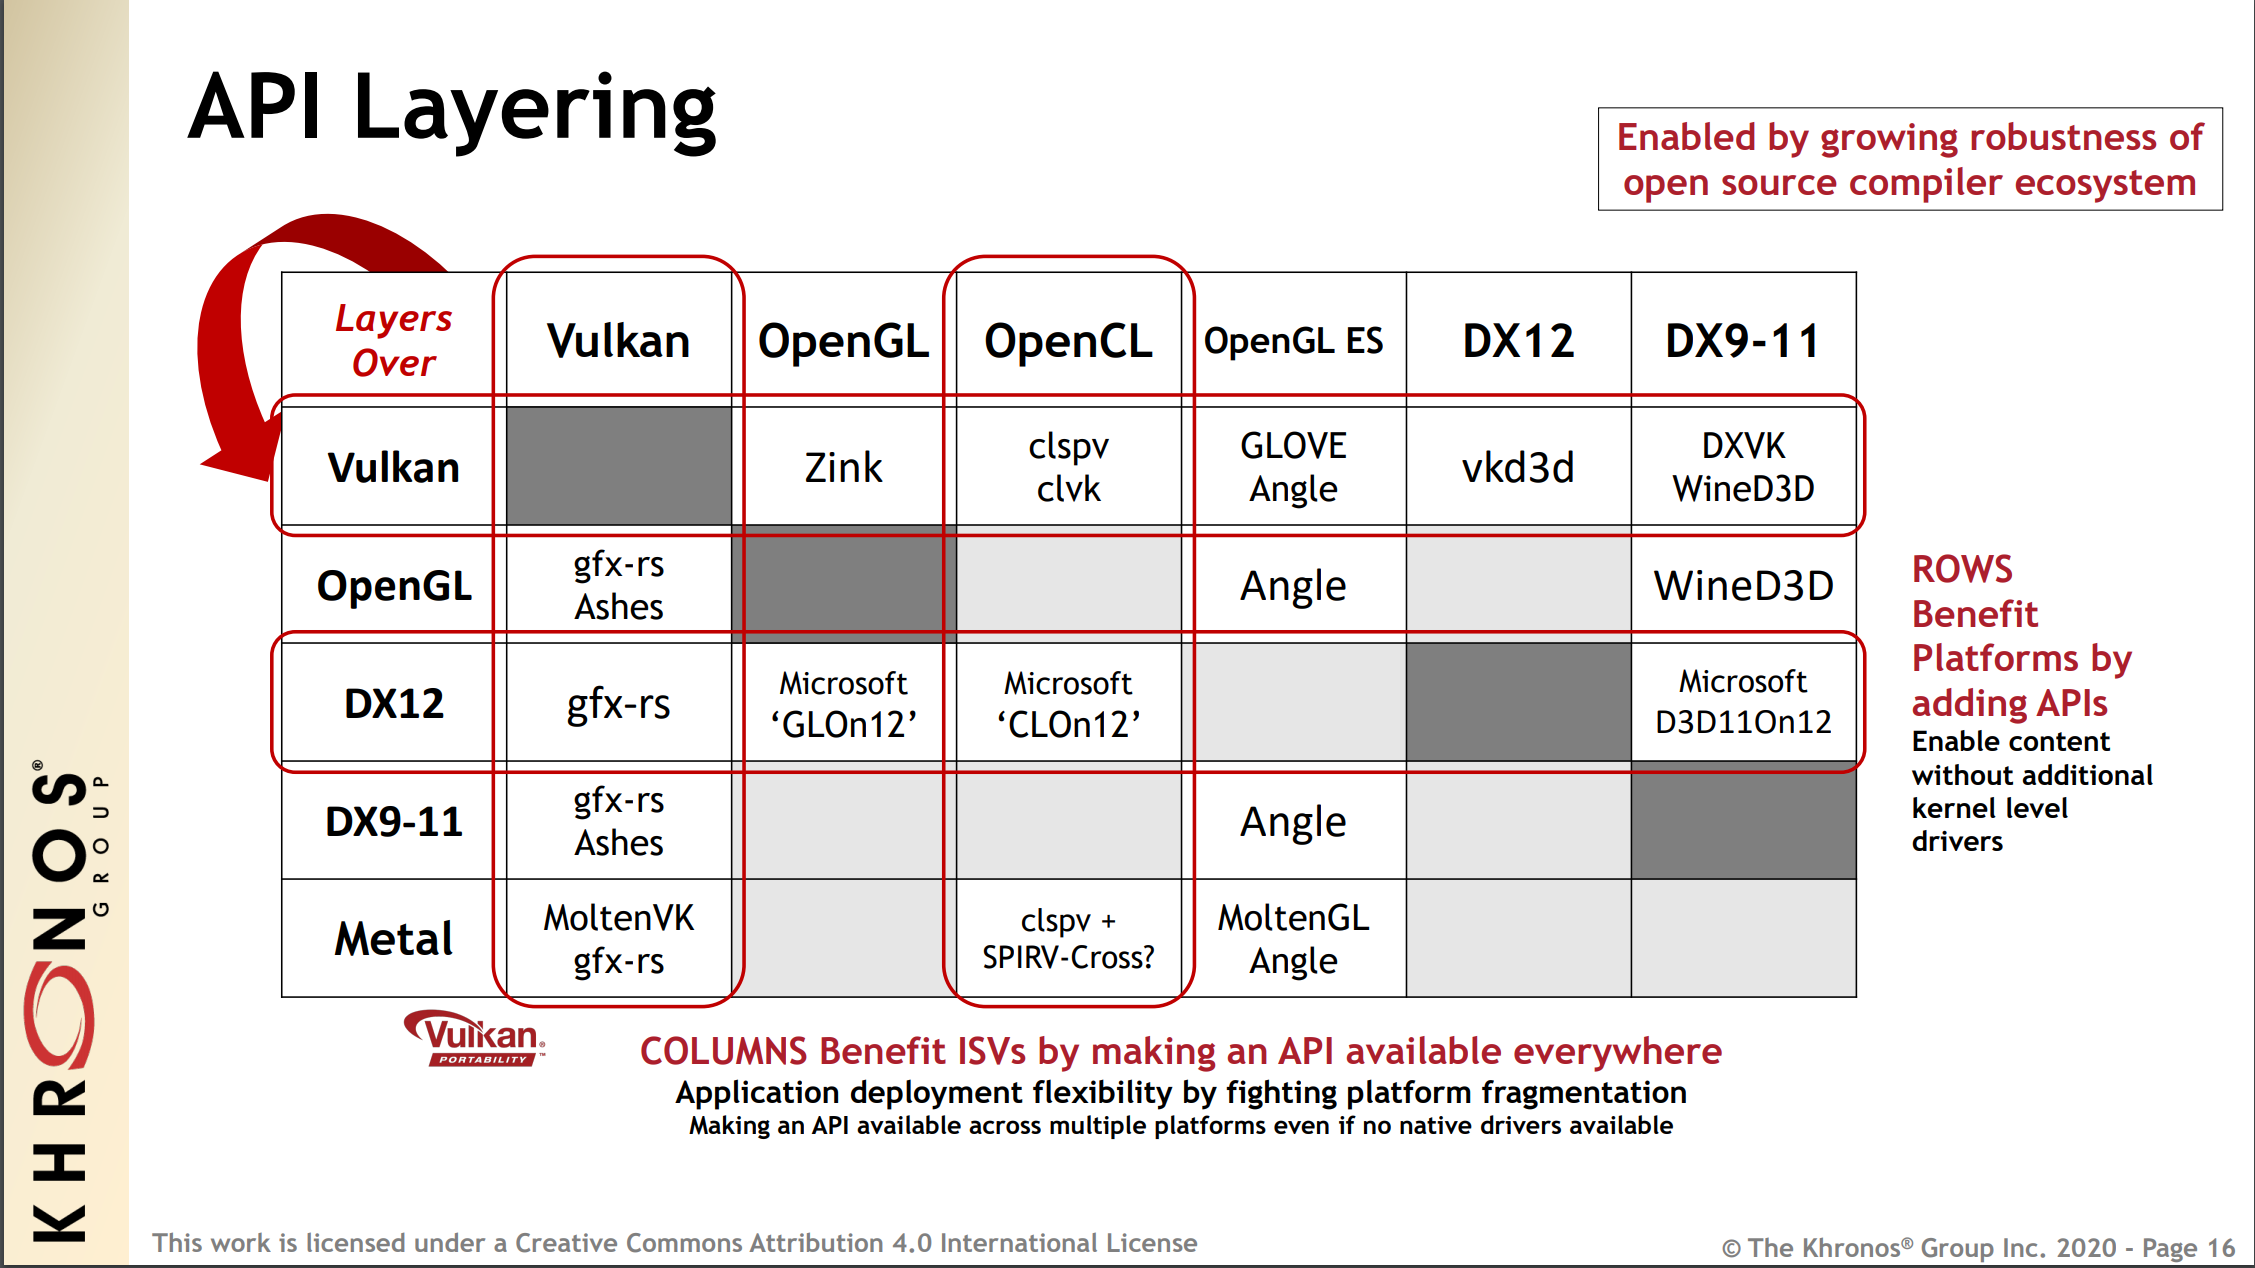
\includegraphics[width=\textwidth]{api_layering}
  \caption{Инструменты эмуляции различных стандартов. Источник: \url{https://www.khronos.org/assets/uploads/apis/OpenCL-3.0-Launch-Apr20.pdf}}
  \label{fig:api_layering}
\end{figure}

\subsubsection{Управление памятью}

Важная функция библиотеки -- управление памятью. Во время исполнения от бинарного
модуля могут поступать запросы на доступ к данным тензоров. Для этого необходимо
отыскать наиболее свежую копию данных, отправить ее на нужное устройство и
пометить этот тензор особым образом, чтобы предотвратить одновременный доступ
с нескольких устройств. Общая схема взаимодействия показана на 
рис.~\ref{fig:memory_management}.

\begin{figure}[h]
  \centering
  
\includegraphics[width=\textwidth]{memory_management}
  \caption{Схема взаимодействия исполняемого модуля и подсистемы управления памятью}
  \label{fig:memory_management}
\end{figure}

Перед запуском все устройства регистрируются в аллокаторе. При этом устройства
могут иметь собственные аллокаторы, а могут переиспользовать системный. Первый
случай возникает, когда у устройства есть собственная модель памяти, не
включающая в себя ОЗУ, например, при исполнении кода на выделенном GPU. Второй --
когда память устройства и ОЗУ -- одно и то же устройство, например, при
исполнении кода на CPU.

При поступлении запроса на выделение памяти под тензор создается специальная
запись, в которой отмечается виртуальный адрес тензора, размер выделяемого
участка памяти, метка версии и устройство, на котором находится эта запись.
Когда поступает запрос на запись в тензор, аллокатор убеждается, что к этой
области памяти больше никто не обращается, находит самую свежую версию записи
и копирует данные на нужное устройство. Если на устройстве закончилось свободное
пространство, аллокатор устройства может выгрузить часть ненужных данных в ОЗУ.
Если и на ОЗУ недостаточно памяти, то часть данных будет выгружена на диск.
Когда поступает уведомление об окончании работы с тензором, запись помечается
как доступная к использованию, но не удаляется с устройства. Это позволяет
избежать лишних копирований данных в случае, если повторный доступ будет
осуществлен на том же устройстве. Аналогичным образом обрабатываются запросы
на чтение тензоров. При этом нескольким устройствам одновременно разрешается
читать один и тот же тензор.

\subsection{Апробация решения}

Для проведения тестов была выбрана модель логистической регрессии. Это статистическая
модель для прогнозирования вероятности возникновения некоторого события путем
сравнения его с логистической кривой. Модель принимает на вход вектор исходных
данных, вектор весовых коэффициэнтов и возвращает ответ в виде вероятности
бинарного события (то есть 1 или 0). Кроме того, в модели задействованы операции
матричного умножения и \textit{сигмоида} -- функция вида \[
  \sigma(x) = \frac{1}{1 + e^{-x}}.
\]
Графическое представление данной модели можно увидеть на рис.~\ref{fig:logreg}.

\begin{figure}[h]
  \centering
  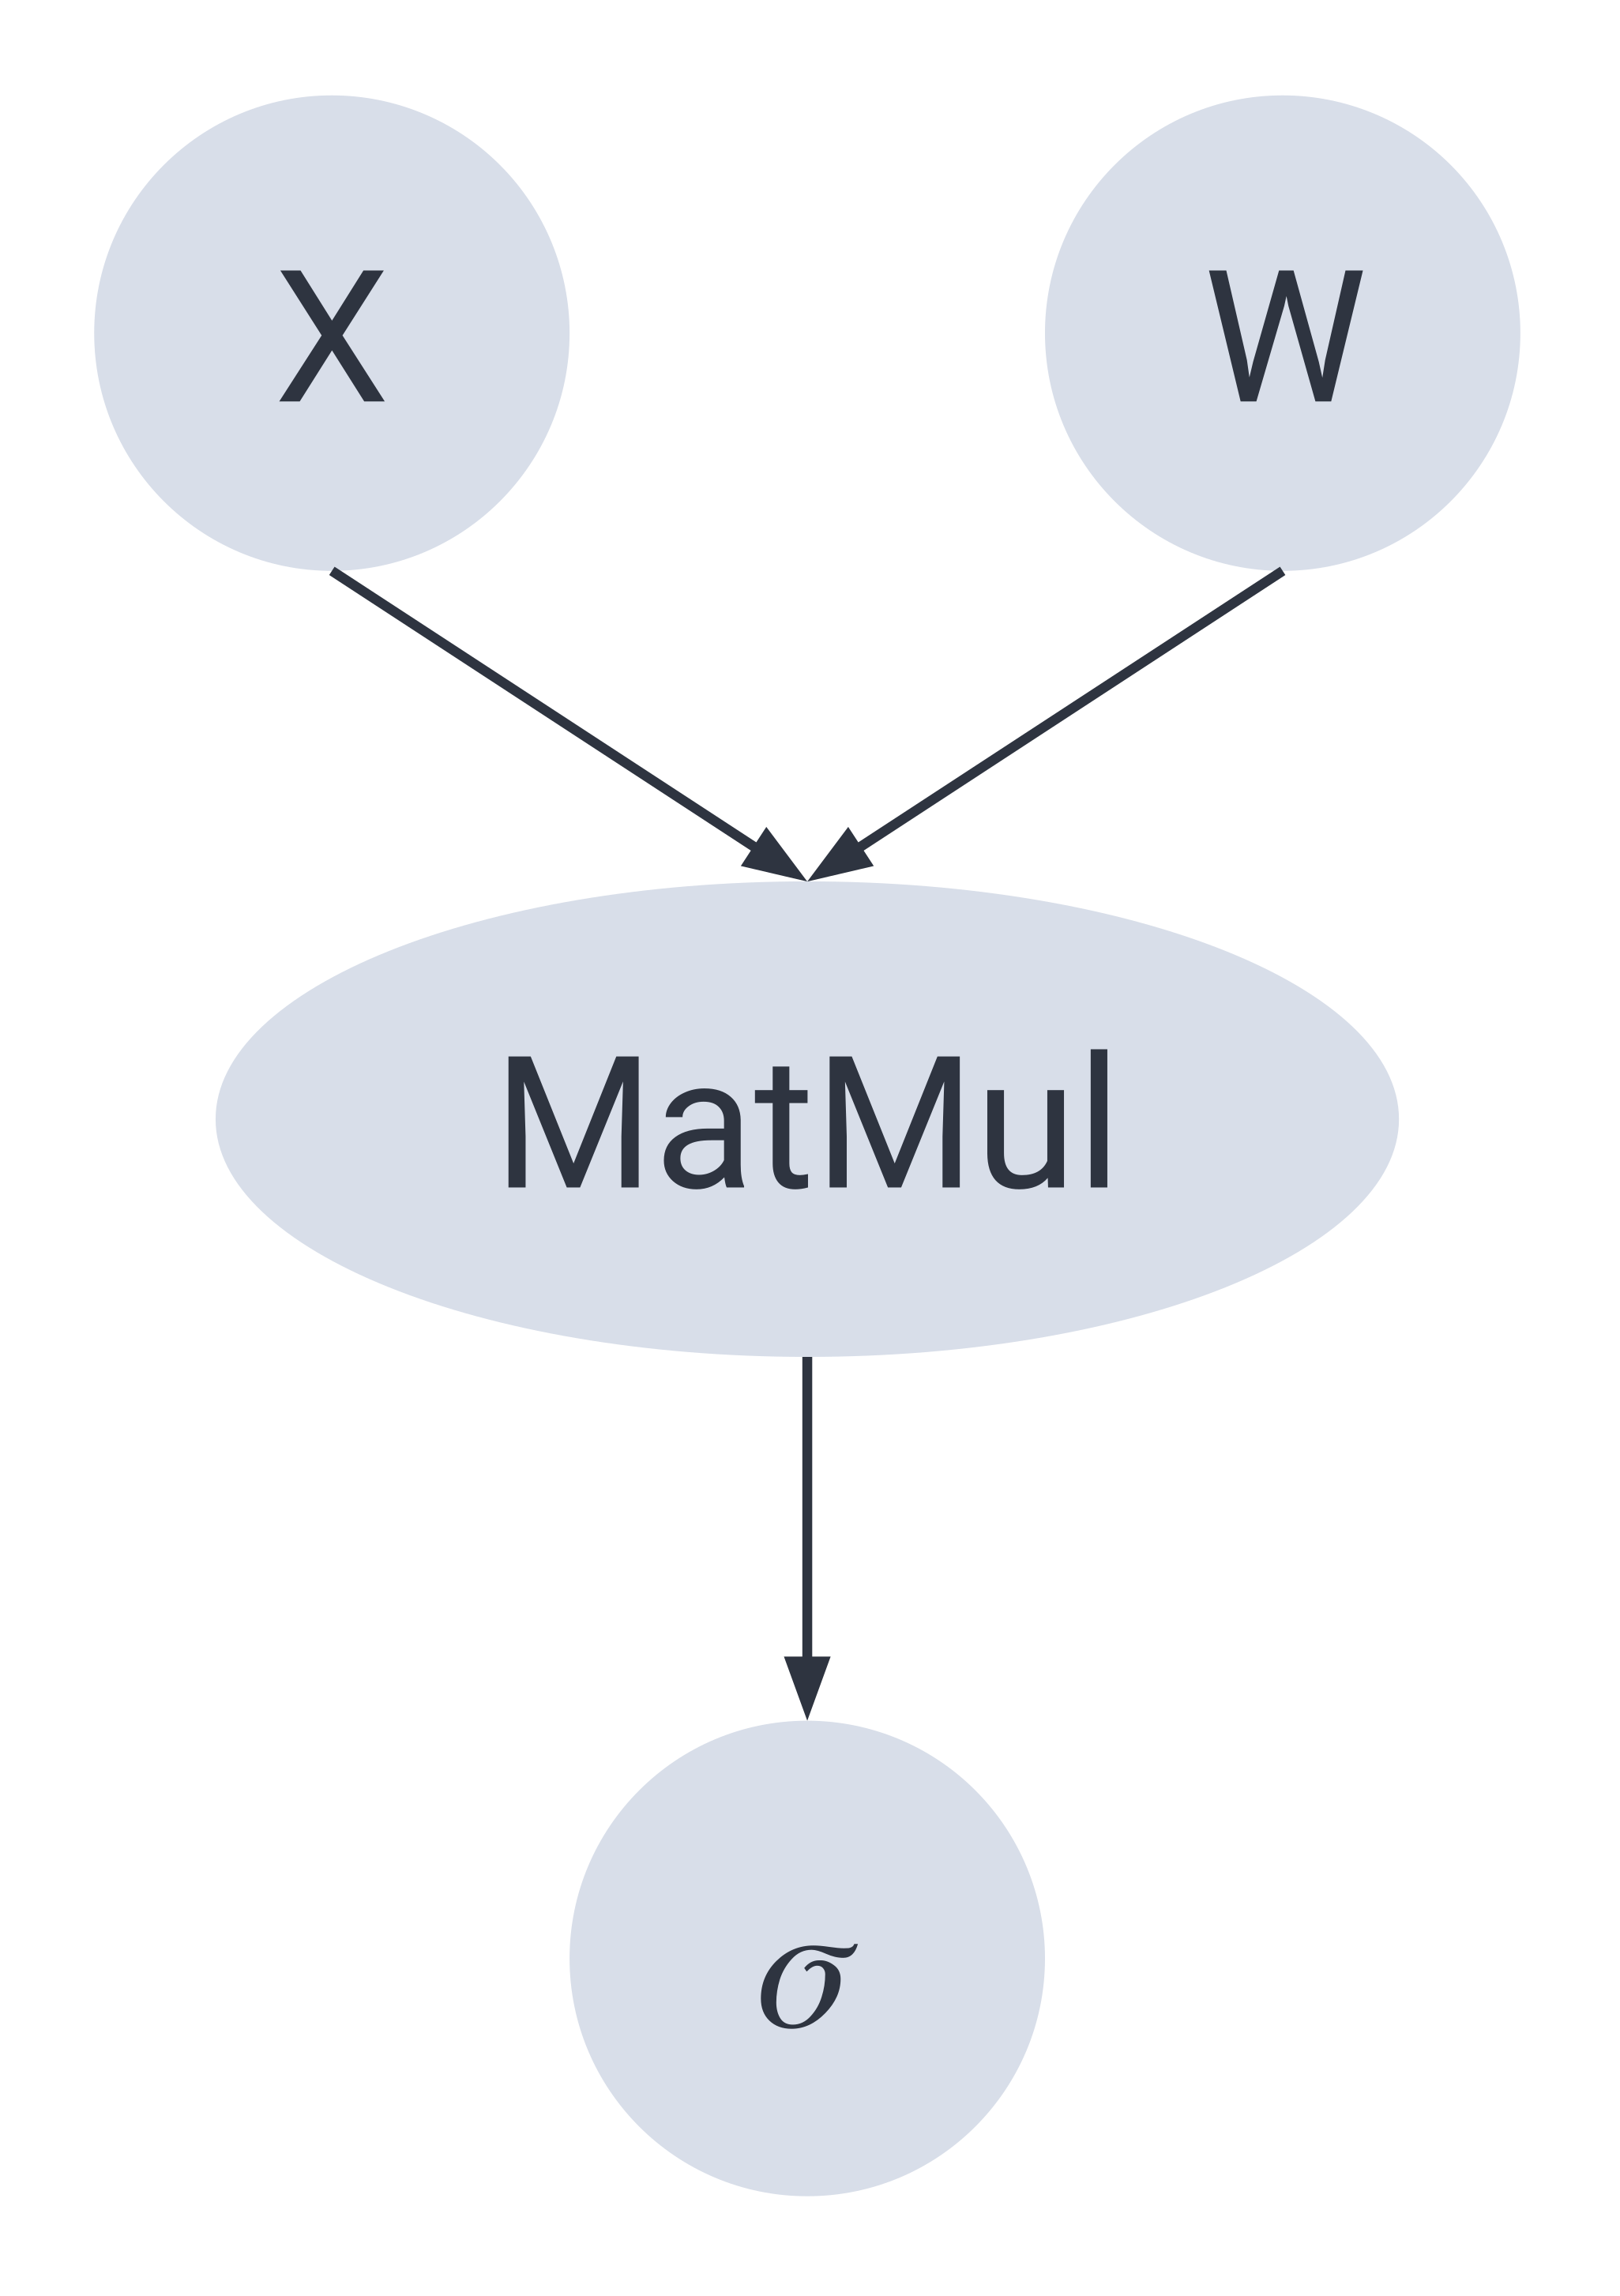
\includegraphics[width=0.2\textwidth]{LogReg}
  \caption{Модель логистической регрессии}
  \label{fig:logreg}
\end{figure}

Сам граф был получен при помощи результатов работы \cite{graph}. Там же подробно
рассмотрен вопрос построения графов для вычисления производной и корректировки
весовых коэффициентов.

На графике~\ref{fig:loss} изображено изменение функции потерь с течением времени.
Уменьшение значения функции потерь говорит об успешном процессе обучения.
\begin{figure}[h]
  \centering
  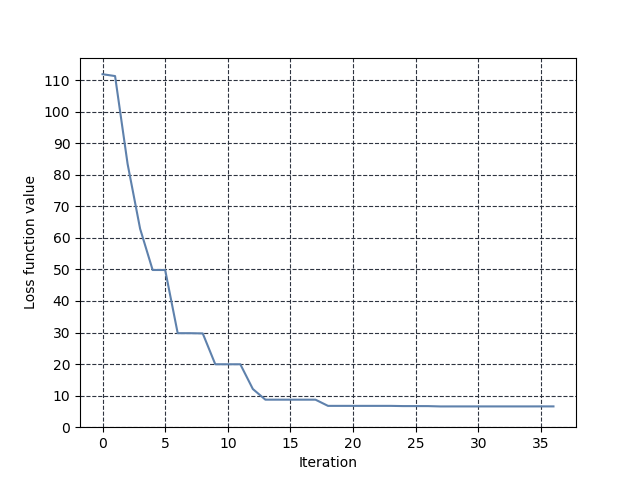
\includegraphics[width=0.8\textwidth]{loss_func_intersect}
  \caption{Функция потерь}
  \label{fig:loss}
\end{figure}

\begin{sidewaysfigure}[ht]
  \begin{subfigure}{.33\textwidth}
    \centering
    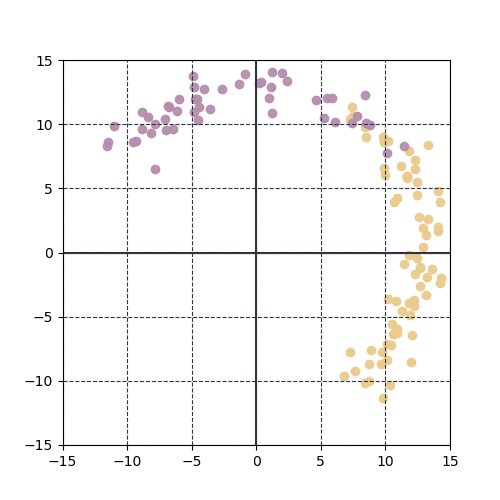
\includegraphics[width=\linewidth]{data_intersect}
    \caption{Исходный набор данных}
  \end{subfigure}
  \begin{subfigure}{.33\textwidth}
    \centering
    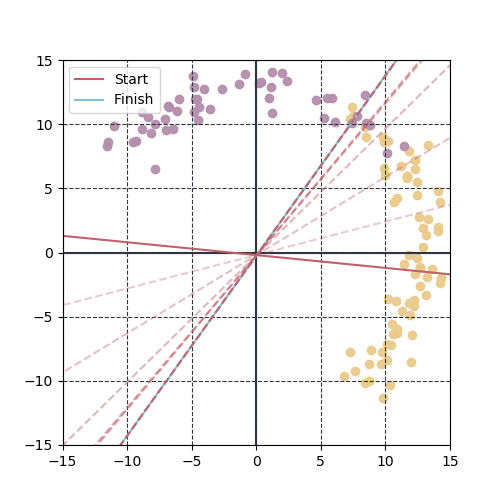
\includegraphics[width=\linewidth]{training_intersect}
    \caption{Поиск решения}
  \end{subfigure}
  \begin{subfigure}{.33\textwidth}
    \centering
    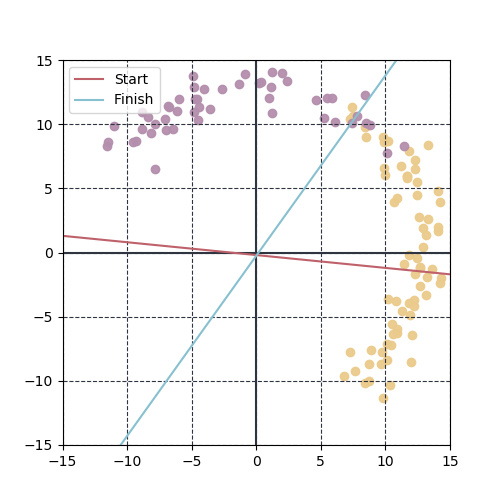
\includegraphics[width=\linewidth]{training_simple_intersect}
    \caption{Конечный результат}
  \end{subfigure}
  \caption{Процесс обучения модели}
  \label{fig:learning}
\end{sidewaysfigure}

Графики на рис.~\ref{fig:learning} демонстрируют процесс поиска корректного
разбиения. Полученные результаты доказывают корректную работу компилятора
графа вычислений.

В листинге~\ref{lst:logreg_graph} Приложения 1 можно ознакомиться с кодом на 
языке диалекта высокого уровня, который получился в результате компиляции модели.

\clearpage
\section{Заключение}

В ходе работы были исследованы фундаментальные концепции лежащие в основе
современных фреймворков искусственного интеллекта, их архитектурные особенности.
Современные библиотеки машинного обучения -- сложные многоуровневые системы.
Они предоставляют различные слои абстракции, необходимые для построения и
развертывания систем на основе глубокого обучения. Предоставляя с одной стороны
простой и понятный интерфейс для исследователя, фреймворки скрывают от пользователя
множество особенностей целевой аппаратной платформе, что позволяет, сосредоточившись
на решении конкретной проблемы, получить достойную производительность на разных
компьютерных системах.

Кроме того, была изучена возможность применения технологий разработки и
построения компиляторов в машинном обучении. Компиляторы -- мост между
программным и аппаратным обеспечением. Многолетний опыт, накопленный в ходе
разработки классических оптимизирующих компиляторов, успешно применяется при
построении фреймворков искусственного интеллекта. Это позволяет одновременно
увеличить производительность на уже поддерживаемых платформах и перенести код
на новые платформы с минимальными изменениями. Более того, машинное обучение
заставило исследователей обобщить используемые методы оптимизации, сделав
их более точными и эффективными. Это, в свою очередь, положительно сказалось
на общей производительности кода, генерируемого компиляторами.

Изученные принципы и технологии легли в основу компилятора графа вычислений, что
стало важным практическим достижением работы. Использование инфраструктуры MLIR 
для построения диалектов промежуточного представления позволяет с одной стророны
сохранять на каждом этапе достаточное количество семантической информации для
проведения необходимых оптимизаций, а сдругой стороны двигаться поступательно,
избавляясь от абстракций, когда в них больше нет нужды. Фреймворк LLVM
зарекомендовал себя как удобное и надежное решение для исследователей в сфере
компиляторных технологий. С его помощью легко построить прототип, который в
дальшейшем можно развить до готового коммерческого решения. Причина этому --
модульная архитектура и большое разнообразие поддерживаемых платформ, а так же
активное сообщество разработчиков, к которому присоединились многие крупные
производители программного и аппаратного обеспечения.

Итоговый программный продукт демонстрирует
новый подход, который только начали брать на вооружение коммерческие компании. 
Он может стать базой для построения эффективных инструментов для задач 
искусственного интеллекта. Будучи центральным компонентом современных 
фреймворков, граф вычислений и его реализация оказывают большое влияние на 
производительность нейронных сетей. Кроме того, графы вычислений могут 
встречаться и в других сферах, например, при глобальной оптимизации функций или
решении дифференциальных уравнений.

В дальнейшем планируется развивать получившийся компилятор графа вычислений.
Среди перспективных направлений более <<агрессивные>> оптимизации, например,
улучшения в области слияния вершин и операций, генерация кода операций с учетом
особенностей аппаратного обеспечения, которое используется для исполнения,
усовершенствованные механизмы планирования исполнения вершин.

Также необходимо отметить, что первоначальная гипотеза об актуальности и важности
синтеза компиляторов и средств машинного обучения подтвердилась. За время
проведения исследования свои наработки и достижения в этой области представили
такие компании как Google (доклад <<MLIR Primer: A Compiler Infrastructure for 
the End of Moore’s Law>> на конференции CGO 2019\footnote{Слайды доступны по 
адресу https://bit.ly/2yDgpG0}) и Intel (доклад <<nGraph Dialect: High-Level 
Graph Optimizations for Deep Learning Workloads>>\footnote{Слайды доступны по 
адресу https://bit.ly/2L7VDks}).


\clearpage
\begingroup
\phantomsection
\addcontentsline{toc}{section}{Приложение 1. Тексты программных модулей}
\section*{Приложение 1. Тексты программных модулей}

\phantomsection
\addcontentsline{toc}{subsection}{П1.1  Результат работы различных стадий компилятора Clang}
\subsection*{П1.1. Результат работы различных стадий компилятора Clang}
\lstinputlisting[label={lst:clang_ast},caption={Текстовое представление Clang AST}]{listings/factorial.ast}

\lstinputlisting[language=llvm,label={lst:llvm_ir_clang},caption={LLVM IR, сгенерированный Clang}]{listings/factorial.ll}

\phantomsection
\addcontentsline{toc}{subsection}{П1.2  Результат работы различных стадий компилятора графа вычислений}
\subsection*{П1.2. Результат работы различных стадий компилятора графа вычислений}
\lstinputlisting[language=athgraph,label={lst:ath_graph_add},caption={Код на языке высокоуровневого диалекта для функции сложения}]{listings/add_graph.mlir}
\lstinputlisting[language=athgraph,label={lst:ath_rt_add},caption={Код на языке низкоуровневого диалекта для функции сложения}]{listings/add_rt.mlir}
\lstinputlisting[language=llvm,label={lst:llvm_add},caption={Итоговый LLVM IR для функции сложения}]{listings/add_llvm.ll}
\lstinputlisting[language=athgraph,label={lst:logreg_graph},caption={Код на языке высокоуровневого диалекта для модели логистической регрессии}]{listings/logreg_graph.mlir}


%% Библиография: отступы и межстрочный интервал
% \makeatletter
% \renewenvironment{thebibliography}[1]
%     {\section*{\refname}
%         \list{\@biblabel{\@arabic\c@enumiv}}
%            {\settowidth\labelwidth{\@biblabel{#1}}
%             \leftmargin\labelsep
%             \itemindent 16.7mm
%             \@openbib@code
%             \usecounter{enumiv}
%             \let\p@enumiv\@empty
%             \renewcommand\theenumiv{\@arabic\c@enumiv}
%         }
%         \setlength{\itemsep}{0pt}
%     }
% \makeatother
\clearpage
\addcontentsline{toc}{section}{Список литературы}
\printbibliography
\end{document}
